\usepackage{ucll-code}
\usepackage{siunitx}
\usepackage{ifthen}

\usetikzlibrary{positioning}

\makeatletter
\def\light@caption@on{on}
\def\light@caption@off{off}
\def\light@caption@neutral{}
\makeatother

\tikzset{
  light/.pic={\draw node[circle,#1,minimum size=7mm,font=\tiny] {\csname light@caption@#1\endcsname};},
  light/.style={draw},
  on/.style={light,fill=yellow},
  off/.style={light,fill=gray!50},
  neutral/.style={light}
}

\title{Data Compression: Huffman}
\author{Fr\'ed\'eric Vogels}

\begin{document}

\begin{frame}
  \titlepage
\end{frame}

\begin{frame}
  \frametitle{Disclaimer}
  \begin{center}
    \Large
    Most examples assume we deal with text,
    but the principles apply to bytes in general
  \end{center}
\end{frame}

{
  \newcommand{\freq}[2]{#1 & \SI{#2}{} \\}
  \begin{frame}
    \frametitle{Letter Frequency in ``A Game of Thrones''}

    \begin{columns}
      \column{4cm}
      \begin{center}
        \begin{tabular}{cc}
          \textbf{Letter} & \textbf{Frequency} \\
          \toprule
          \freq{E}{154148}
          \freq{T}{101753}
          \freq{A}{98313}
          \freq{O}{92254}
          \freq{H}{86942}
          \freq{N}{81018}
          \freq{S}{80389}
          \freq{R}{78068}
          \freq{I}{71945}
          \freq{D}{65816}
          \freq{L}{53882}
          \freq{W}{32485}
          \freq{U}{29804}
        \end{tabular}
      \end{center}

      \column{4cm}
      \begin{center}
        \begin{tabular}{cc}
          \textbf{Letter} & \textbf{Frequency} \\
          \toprule
          \freq{M}{29129}
          \freq{G}{27193}
          \freq{Y}{25888}
          \freq{F}{25074}
          \freq{C}{22459}
          \freq{B}{20154}
          \freq{P}{14831}
          \freq{K}{14469}
          \freq{V}{9068}
          \freq{J}{2513}
          \freq{Q}{1050}
          \freq{Z}{599}
          \freq{X}{591}
        \end{tabular}
      \end{center}
    \end{columns}
  \end{frame}
}

\begin{frame}
  \frametitle{Bits vs Letter Frequency}
  \begin{itemize}
    \item Each letter is represented by a unique 8 bit code (ASCII)
    \item The letter E is used 261$\times$ more often than X
    \item It would make more sense to use less bits for E than for~X
  \end{itemize}
\end{frame}

\begin{frame}
  \frametitle{Using Less Bits}
  \begin{itemize}
    \item Say we use 4 bits for E: \texttt{0101}
    \item EE corresponds to \texttt{01010101}
    \item Problem: {\tt U} is also represented by \texttt{01010101}
    \item Decompressor can't know whether you mean EE of U
    \item It is impossible to simply assign a shorter code to E without introducing ambiguities
    \item In order to encode E with less bits, we need to change more than just E's code
  \end{itemize}
\end{frame}

\begin{frame}
  \frametitle{How To Build An Unambiguous Encoding}
  \begin{itemize}
    \item Visualising helps
    \item First, we represent our codes by a tree
    \item Next, we find out what operations we can apply on a tree
  \end{itemize}
\end{frame}

\begin{frame}
  \frametitle{How To Build An Unambiguous Encoding}
  \begin{center}
    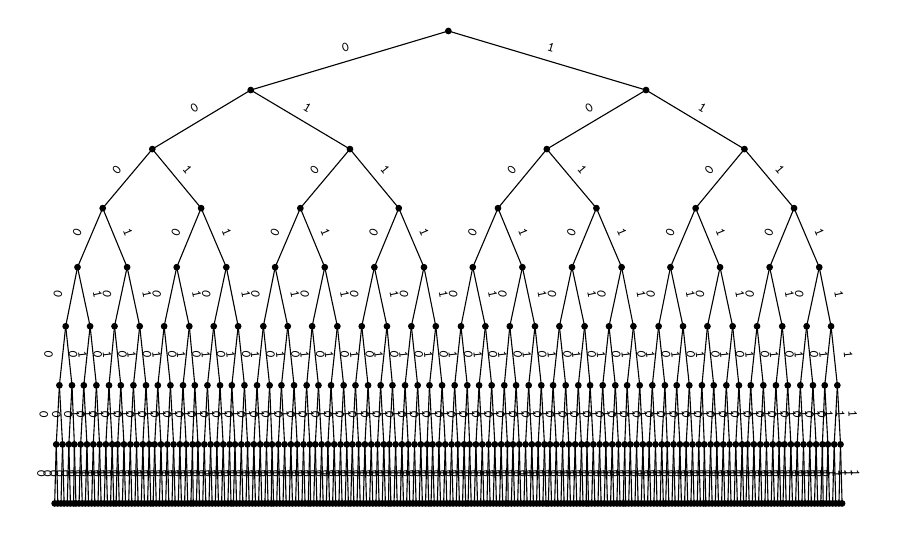
\begin{tikzpicture}
      \draw[fill] (0.0,0.0) circle[radius=1pt];
      \draw[fill] (0.04,0.0) circle[radius=1pt];
      \draw[fill] (0.08,0.0) circle[radius=1pt];
      \draw[fill] (0.12,0.0) circle[radius=1pt];
      \draw[fill] (0.16,0.0) circle[radius=1pt];
      \draw[fill] (0.2,0.0) circle[radius=1pt];
      \draw[fill] (0.24,0.0) circle[radius=1pt];
      \draw[fill] (0.27,0.0) circle[radius=1pt];
      \draw[fill] (0.31,0.0) circle[radius=1pt];
      \draw[fill] (0.35,0.0) circle[radius=1pt];
      \draw[fill] (0.39,0.0) circle[radius=1pt];
      \draw[fill] (0.43,0.0) circle[radius=1pt];
      \draw[fill] (0.47,0.0) circle[radius=1pt];
      \draw[fill] (0.51,0.0) circle[radius=1pt];
      \draw[fill] (0.55,0.0) circle[radius=1pt];
      \draw[fill] (0.59,0.0) circle[radius=1pt];
      \draw[fill] (0.63,0.0) circle[radius=1pt];
      \draw[fill] (0.67,0.0) circle[radius=1pt];
      \draw[fill] (0.71,0.0) circle[radius=1pt];
      \draw[fill] (0.75,0.0) circle[radius=1pt];
      \draw[fill] (0.78,0.0) circle[radius=1pt];
      \draw[fill] (0.82,0.0) circle[radius=1pt];
      \draw[fill] (0.86,0.0) circle[radius=1pt];
      \draw[fill] (0.9,0.0) circle[radius=1pt];
      \draw[fill] (0.94,0.0) circle[radius=1pt];
      \draw[fill] (0.98,0.0) circle[radius=1pt];
      \draw[fill] (1.02,0.0) circle[radius=1pt];
      \draw[fill] (1.06,0.0) circle[radius=1pt];
      \draw[fill] (1.1,0.0) circle[radius=1pt];
      \draw[fill] (1.14,0.0) circle[radius=1pt];
      \draw[fill] (1.18,0.0) circle[radius=1pt];
      \draw[fill] (1.22,0.0) circle[radius=1pt];
      \draw[fill] (1.25,0.0) circle[radius=1pt];
      \draw[fill] (1.29,0.0) circle[radius=1pt];
      \draw[fill] (1.33,0.0) circle[radius=1pt];
      \draw[fill] (1.37,0.0) circle[radius=1pt];
      \draw[fill] (1.41,0.0) circle[radius=1pt];
      \draw[fill] (1.45,0.0) circle[radius=1pt];
      \draw[fill] (1.49,0.0) circle[radius=1pt];
      \draw[fill] (1.53,0.0) circle[radius=1pt];
      \draw[fill] (1.57,0.0) circle[radius=1pt];
      \draw[fill] (1.61,0.0) circle[radius=1pt];
      \draw[fill] (1.65,0.0) circle[radius=1pt];
      \draw[fill] (1.69,0.0) circle[radius=1pt];
      \draw[fill] (1.73,0.0) circle[radius=1pt];
      \draw[fill] (1.76,0.0) circle[radius=1pt];
      \draw[fill] (1.8,0.0) circle[radius=1pt];
      \draw[fill] (1.84,0.0) circle[radius=1pt];
      \draw[fill] (1.88,0.0) circle[radius=1pt];
      \draw[fill] (1.92,0.0) circle[radius=1pt];
      \draw[fill] (1.96,0.0) circle[radius=1pt];
      \draw[fill] (2.0,0.0) circle[radius=1pt];
      \draw[fill] (2.04,0.0) circle[radius=1pt];
      \draw[fill] (2.08,0.0) circle[radius=1pt];
      \draw[fill] (2.12,0.0) circle[radius=1pt];
      \draw[fill] (2.16,0.0) circle[radius=1pt];
      \draw[fill] (2.2,0.0) circle[radius=1pt];
      \draw[fill] (2.24,0.0) circle[radius=1pt];
      \draw[fill] (2.27,0.0) circle[radius=1pt];
      \draw[fill] (2.31,0.0) circle[radius=1pt];
      \draw[fill] (2.35,0.0) circle[radius=1pt];
      \draw[fill] (2.39,0.0) circle[radius=1pt];
      \draw[fill] (2.43,0.0) circle[radius=1pt];
      \draw[fill] (2.47,0.0) circle[radius=1pt];
      \draw[fill] (2.51,0.0) circle[radius=1pt];
      \draw[fill] (2.55,0.0) circle[radius=1pt];
      \draw[fill] (2.59,0.0) circle[radius=1pt];
      \draw[fill] (2.63,0.0) circle[radius=1pt];
      \draw[fill] (2.67,0.0) circle[radius=1pt];
      \draw[fill] (2.71,0.0) circle[radius=1pt];
      \draw[fill] (2.75,0.0) circle[radius=1pt];
      \draw[fill] (2.78,0.0) circle[radius=1pt];
      \draw[fill] (2.82,0.0) circle[radius=1pt];
      \draw[fill] (2.86,0.0) circle[radius=1pt];
      \draw[fill] (2.9,0.0) circle[radius=1pt];
      \draw[fill] (2.94,0.0) circle[radius=1pt];
      \draw[fill] (2.98,0.0) circle[radius=1pt];
      \draw[fill] (3.02,0.0) circle[radius=1pt];
      \draw[fill] (3.06,0.0) circle[radius=1pt];
      \draw[fill] (3.1,0.0) circle[radius=1pt];
      \draw[fill] (3.14,0.0) circle[radius=1pt];
      \draw[fill] (3.18,0.0) circle[radius=1pt];
      \draw[fill] (3.22,0.0) circle[radius=1pt];
      \draw[fill] (3.25,0.0) circle[radius=1pt];
      \draw[fill] (3.29,0.0) circle[radius=1pt];
      \draw[fill] (3.33,0.0) circle[radius=1pt];
      \draw[fill] (3.37,0.0) circle[radius=1pt];
      \draw[fill] (3.41,0.0) circle[radius=1pt];
      \draw[fill] (3.45,0.0) circle[radius=1pt];
      \draw[fill] (3.49,0.0) circle[radius=1pt];
      \draw[fill] (3.53,0.0) circle[radius=1pt];
      \draw[fill] (3.57,0.0) circle[radius=1pt];
      \draw[fill] (3.61,0.0) circle[radius=1pt];
      \draw[fill] (3.65,0.0) circle[radius=1pt];
      \draw[fill] (3.69,0.0) circle[radius=1pt];
      \draw[fill] (3.73,0.0) circle[radius=1pt];
      \draw[fill] (3.76,0.0) circle[radius=1pt];
      \draw[fill] (3.8,0.0) circle[radius=1pt];
      \draw[fill] (3.84,0.0) circle[radius=1pt];
      \draw[fill] (3.88,0.0) circle[radius=1pt];
      \draw[fill] (3.92,0.0) circle[radius=1pt];
      \draw[fill] (3.96,0.0) circle[radius=1pt];
      \draw[fill] (4.0,0.0) circle[radius=1pt];
      \draw[fill] (4.04,0.0) circle[radius=1pt];
      \draw[fill] (4.08,0.0) circle[radius=1pt];
      \draw[fill] (4.12,0.0) circle[radius=1pt];
      \draw[fill] (4.16,0.0) circle[radius=1pt];
      \draw[fill] (4.2,0.0) circle[radius=1pt];
      \draw[fill] (4.24,0.0) circle[radius=1pt];
      \draw[fill] (4.27,0.0) circle[radius=1pt];
      \draw[fill] (4.31,0.0) circle[radius=1pt];
      \draw[fill] (4.35,0.0) circle[radius=1pt];
      \draw[fill] (4.39,0.0) circle[radius=1pt];
      \draw[fill] (4.43,0.0) circle[radius=1pt];
      \draw[fill] (4.47,0.0) circle[radius=1pt];
      \draw[fill] (4.51,0.0) circle[radius=1pt];
      \draw[fill] (4.55,0.0) circle[radius=1pt];
      \draw[fill] (4.59,0.0) circle[radius=1pt];
      \draw[fill] (4.63,0.0) circle[radius=1pt];
      \draw[fill] (4.67,0.0) circle[radius=1pt];
      \draw[fill] (4.71,0.0) circle[radius=1pt];
      \draw[fill] (4.75,0.0) circle[radius=1pt];
      \draw[fill] (4.78,0.0) circle[radius=1pt];
      \draw[fill] (4.82,0.0) circle[radius=1pt];
      \draw[fill] (4.86,0.0) circle[radius=1pt];
      \draw[fill] (4.9,0.0) circle[radius=1pt];
      \draw[fill] (4.94,0.0) circle[radius=1pt];
      \draw[fill] (4.98,0.0) circle[radius=1pt];
      \draw[fill] (5.02,0.0) circle[radius=1pt];
      \draw[fill] (5.06,0.0) circle[radius=1pt];
      \draw[fill] (5.1,0.0) circle[radius=1pt];
      \draw[fill] (5.14,0.0) circle[radius=1pt];
      \draw[fill] (5.18,0.0) circle[radius=1pt];
      \draw[fill] (5.22,0.0) circle[radius=1pt];
      \draw[fill] (5.25,0.0) circle[radius=1pt];
      \draw[fill] (5.29,0.0) circle[radius=1pt];
      \draw[fill] (5.33,0.0) circle[radius=1pt];
      \draw[fill] (5.37,0.0) circle[radius=1pt];
      \draw[fill] (5.41,0.0) circle[radius=1pt];
      \draw[fill] (5.45,0.0) circle[radius=1pt];
      \draw[fill] (5.49,0.0) circle[radius=1pt];
      \draw[fill] (5.53,0.0) circle[radius=1pt];
      \draw[fill] (5.57,0.0) circle[radius=1pt];
      \draw[fill] (5.61,0.0) circle[radius=1pt];
      \draw[fill] (5.65,0.0) circle[radius=1pt];
      \draw[fill] (5.69,0.0) circle[radius=1pt];
      \draw[fill] (5.73,0.0) circle[radius=1pt];
      \draw[fill] (5.76,0.0) circle[radius=1pt];
      \draw[fill] (5.8,0.0) circle[radius=1pt];
      \draw[fill] (5.84,0.0) circle[radius=1pt];
      \draw[fill] (5.88,0.0) circle[radius=1pt];
      \draw[fill] (5.92,0.0) circle[radius=1pt];
      \draw[fill] (5.96,0.0) circle[radius=1pt];
      \draw[fill] (6.0,0.0) circle[radius=1pt];
      \draw[fill] (6.04,0.0) circle[radius=1pt];
      \draw[fill] (6.08,0.0) circle[radius=1pt];
      \draw[fill] (6.12,0.0) circle[radius=1pt];
      \draw[fill] (6.16,0.0) circle[radius=1pt];
      \draw[fill] (6.2,0.0) circle[radius=1pt];
      \draw[fill] (6.24,0.0) circle[radius=1pt];
      \draw[fill] (6.27,0.0) circle[radius=1pt];
      \draw[fill] (6.31,0.0) circle[radius=1pt];
      \draw[fill] (6.35,0.0) circle[radius=1pt];
      \draw[fill] (6.39,0.0) circle[radius=1pt];
      \draw[fill] (6.43,0.0) circle[radius=1pt];
      \draw[fill] (6.47,0.0) circle[radius=1pt];
      \draw[fill] (6.51,0.0) circle[radius=1pt];
      \draw[fill] (6.55,0.0) circle[radius=1pt];
      \draw[fill] (6.59,0.0) circle[radius=1pt];
      \draw[fill] (6.63,0.0) circle[radius=1pt];
      \draw[fill] (6.67,0.0) circle[radius=1pt];
      \draw[fill] (6.71,0.0) circle[radius=1pt];
      \draw[fill] (6.75,0.0) circle[radius=1pt];
      \draw[fill] (6.78,0.0) circle[radius=1pt];
      \draw[fill] (6.82,0.0) circle[radius=1pt];
      \draw[fill] (6.86,0.0) circle[radius=1pt];
      \draw[fill] (6.9,0.0) circle[radius=1pt];
      \draw[fill] (6.94,0.0) circle[radius=1pt];
      \draw[fill] (6.98,0.0) circle[radius=1pt];
      \draw[fill] (7.02,0.0) circle[radius=1pt];
      \draw[fill] (7.06,0.0) circle[radius=1pt];
      \draw[fill] (7.1,0.0) circle[radius=1pt];
      \draw[fill] (7.14,0.0) circle[radius=1pt];
      \draw[fill] (7.18,0.0) circle[radius=1pt];
      \draw[fill] (7.22,0.0) circle[radius=1pt];
      \draw[fill] (7.25,0.0) circle[radius=1pt];
      \draw[fill] (7.29,0.0) circle[radius=1pt];
      \draw[fill] (7.33,0.0) circle[radius=1pt];
      \draw[fill] (7.37,0.0) circle[radius=1pt];
      \draw[fill] (7.41,0.0) circle[radius=1pt];
      \draw[fill] (7.45,0.0) circle[radius=1pt];
      \draw[fill] (7.49,0.0) circle[radius=1pt];
      \draw[fill] (7.53,0.0) circle[radius=1pt];
      \draw[fill] (7.57,0.0) circle[radius=1pt];
      \draw[fill] (7.61,0.0) circle[radius=1pt];
      \draw[fill] (7.65,0.0) circle[radius=1pt];
      \draw[fill] (7.69,0.0) circle[radius=1pt];
      \draw[fill] (7.73,0.0) circle[radius=1pt];
      \draw[fill] (7.76,0.0) circle[radius=1pt];
      \draw[fill] (7.8,0.0) circle[radius=1pt];
      \draw[fill] (7.84,0.0) circle[radius=1pt];
      \draw[fill] (7.88,0.0) circle[radius=1pt];
      \draw[fill] (7.92,0.0) circle[radius=1pt];
      \draw[fill] (7.96,0.0) circle[radius=1pt];
      \draw[fill] (8.0,0.0) circle[radius=1pt];
      \draw[fill] (8.04,0.0) circle[radius=1pt];
      \draw[fill] (8.08,0.0) circle[radius=1pt];
      \draw[fill] (8.12,0.0) circle[radius=1pt];
      \draw[fill] (8.16,0.0) circle[radius=1pt];
      \draw[fill] (8.2,0.0) circle[radius=1pt];
      \draw[fill] (8.24,0.0) circle[radius=1pt];
      \draw[fill] (8.27,0.0) circle[radius=1pt];
      \draw[fill] (8.31,0.0) circle[radius=1pt];
      \draw[fill] (8.35,0.0) circle[radius=1pt];
      \draw[fill] (8.39,0.0) circle[radius=1pt];
      \draw[fill] (8.43,0.0) circle[radius=1pt];
      \draw[fill] (8.47,0.0) circle[radius=1pt];
      \draw[fill] (8.51,0.0) circle[radius=1pt];
      \draw[fill] (8.55,0.0) circle[radius=1pt];
      \draw[fill] (8.59,0.0) circle[radius=1pt];
      \draw[fill] (8.63,0.0) circle[radius=1pt];
      \draw[fill] (8.67,0.0) circle[radius=1pt];
      \draw[fill] (8.71,0.0) circle[radius=1pt];
      \draw[fill] (8.75,0.0) circle[radius=1pt];
      \draw[fill] (8.78,0.0) circle[radius=1pt];
      \draw[fill] (8.82,0.0) circle[radius=1pt];
      \draw[fill] (8.86,0.0) circle[radius=1pt];
      \draw[fill] (8.9,0.0) circle[radius=1pt];
      \draw[fill] (8.94,0.0) circle[radius=1pt];
      \draw[fill] (8.98,0.0) circle[radius=1pt];
      \draw[fill] (9.02,0.0) circle[radius=1pt];
      \draw[fill] (9.06,0.0) circle[radius=1pt];
      \draw[fill] (9.1,0.0) circle[radius=1pt];
      \draw[fill] (9.14,0.0) circle[radius=1pt];
      \draw[fill] (9.18,0.0) circle[radius=1pt];
      \draw[fill] (9.22,0.0) circle[radius=1pt];
      \draw[fill] (9.25,0.0) circle[radius=1pt];
      \draw[fill] (9.29,0.0) circle[radius=1pt];
      \draw[fill] (9.33,0.0) circle[radius=1pt];
      \draw[fill] (9.37,0.0) circle[radius=1pt];
      \draw[fill] (9.41,0.0) circle[radius=1pt];
      \draw[fill] (9.45,0.0) circle[radius=1pt];
      \draw[fill] (9.49,0.0) circle[radius=1pt];
      \draw[fill] (9.53,0.0) circle[radius=1pt];
      \draw[fill] (9.57,0.0) circle[radius=1pt];
      \draw[fill] (9.61,0.0) circle[radius=1pt];
      \draw[fill] (9.65,0.0) circle[radius=1pt];
      \draw[fill] (9.69,0.0) circle[radius=1pt];
      \draw[fill] (9.73,0.0) circle[radius=1pt];
      \draw[fill] (9.76,0.0) circle[radius=1pt];
      \draw[fill] (9.8,0.0) circle[radius=1pt];
      \draw[fill] (9.84,0.0) circle[radius=1pt];
      \draw[fill] (9.88,0.0) circle[radius=1pt];
      \draw[fill] (9.92,0.0) circle[radius=1pt];
      \draw[fill] (9.96,0.0) circle[radius=1pt];
      \draw[fill] (10.0,0.0) circle[radius=1pt];
      \draw (0.0,0.0) -- (0.02,0.75) node[midway,above,sloped,font=\tiny] {\tt 0};
      \draw (0.04,0.0) -- (0.02,0.75) node[midway,above,sloped,font=\tiny] {\tt 1};
      \draw (0.08,0.0) -- (0.1,0.75) node[midway,above,sloped,font=\tiny] {\tt 0};
      \draw (0.12,0.0) -- (0.1,0.75) node[midway,above,sloped,font=\tiny] {\tt 1};
      \draw (0.16,0.0) -- (0.18,0.75) node[midway,above,sloped,font=\tiny] {\tt 0};
      \draw (0.2,0.0) -- (0.18,0.75) node[midway,above,sloped,font=\tiny] {\tt 1};
      \draw (0.24,0.0) -- (0.25,0.75) node[midway,above,sloped,font=\tiny] {\tt 0};
      \draw (0.27,0.0) -- (0.25,0.75) node[midway,above,sloped,font=\tiny] {\tt 1};
      \draw (0.31,0.0) -- (0.33,0.75) node[midway,above,sloped,font=\tiny] {\tt 0};
      \draw (0.35,0.0) -- (0.33,0.75) node[midway,above,sloped,font=\tiny] {\tt 1};
      \draw (0.39,0.0) -- (0.41,0.75) node[midway,above,sloped,font=\tiny] {\tt 0};
      \draw (0.43,0.0) -- (0.41,0.75) node[midway,above,sloped,font=\tiny] {\tt 1};
      \draw (0.47,0.0) -- (0.49,0.75) node[midway,above,sloped,font=\tiny] {\tt 0};
      \draw (0.51,0.0) -- (0.49,0.75) node[midway,above,sloped,font=\tiny] {\tt 1};
      \draw (0.55,0.0) -- (0.57,0.75) node[midway,above,sloped,font=\tiny] {\tt 0};
      \draw (0.59,0.0) -- (0.57,0.75) node[midway,above,sloped,font=\tiny] {\tt 1};
      \draw (0.63,0.0) -- (0.65,0.75) node[midway,above,sloped,font=\tiny] {\tt 0};
      \draw (0.67,0.0) -- (0.65,0.75) node[midway,above,sloped,font=\tiny] {\tt 1};
      \draw (0.71,0.0) -- (0.73,0.75) node[midway,above,sloped,font=\tiny] {\tt 0};
      \draw (0.75,0.0) -- (0.73,0.75) node[midway,above,sloped,font=\tiny] {\tt 1};
      \draw (0.78,0.0) -- (0.8,0.75) node[midway,above,sloped,font=\tiny] {\tt 0};
      \draw (0.82,0.0) -- (0.8,0.75) node[midway,above,sloped,font=\tiny] {\tt 1};
      \draw (0.86,0.0) -- (0.88,0.75) node[midway,above,sloped,font=\tiny] {\tt 0};
      \draw (0.9,0.0) -- (0.88,0.75) node[midway,above,sloped,font=\tiny] {\tt 1};
      \draw (0.94,0.0) -- (0.96,0.75) node[midway,above,sloped,font=\tiny] {\tt 0};
      \draw (0.98,0.0) -- (0.96,0.75) node[midway,above,sloped,font=\tiny] {\tt 1};
      \draw (1.02,0.0) -- (1.04,0.75) node[midway,above,sloped,font=\tiny] {\tt 0};
      \draw (1.06,0.0) -- (1.04,0.75) node[midway,above,sloped,font=\tiny] {\tt 1};
      \draw (1.1,0.0) -- (1.12,0.75) node[midway,above,sloped,font=\tiny] {\tt 0};
      \draw (1.14,0.0) -- (1.12,0.75) node[midway,above,sloped,font=\tiny] {\tt 1};
      \draw (1.18,0.0) -- (1.2,0.75) node[midway,above,sloped,font=\tiny] {\tt 0};
      \draw (1.22,0.0) -- (1.2,0.75) node[midway,above,sloped,font=\tiny] {\tt 1};
      \draw (1.25,0.0) -- (1.27,0.75) node[midway,above,sloped,font=\tiny] {\tt 0};
      \draw (1.29,0.0) -- (1.27,0.75) node[midway,above,sloped,font=\tiny] {\tt 1};
      \draw (1.33,0.0) -- (1.35,0.75) node[midway,above,sloped,font=\tiny] {\tt 0};
      \draw (1.37,0.0) -- (1.35,0.75) node[midway,above,sloped,font=\tiny] {\tt 1};
      \draw (1.41,0.0) -- (1.43,0.75) node[midway,above,sloped,font=\tiny] {\tt 0};
      \draw (1.45,0.0) -- (1.43,0.75) node[midway,above,sloped,font=\tiny] {\tt 1};
      \draw (1.49,0.0) -- (1.51,0.75) node[midway,above,sloped,font=\tiny] {\tt 0};
      \draw (1.53,0.0) -- (1.51,0.75) node[midway,above,sloped,font=\tiny] {\tt 1};
      \draw (1.57,0.0) -- (1.59,0.75) node[midway,above,sloped,font=\tiny] {\tt 0};
      \draw (1.61,0.0) -- (1.59,0.75) node[midway,above,sloped,font=\tiny] {\tt 1};
      \draw (1.65,0.0) -- (1.67,0.75) node[midway,above,sloped,font=\tiny] {\tt 0};
      \draw (1.69,0.0) -- (1.67,0.75) node[midway,above,sloped,font=\tiny] {\tt 1};
      \draw (1.73,0.0) -- (1.75,0.75) node[midway,above,sloped,font=\tiny] {\tt 0};
      \draw (1.76,0.0) -- (1.75,0.75) node[midway,above,sloped,font=\tiny] {\tt 1};
      \draw (1.8,0.0) -- (1.82,0.75) node[midway,above,sloped,font=\tiny] {\tt 0};
      \draw (1.84,0.0) -- (1.82,0.75) node[midway,above,sloped,font=\tiny] {\tt 1};
      \draw (1.88,0.0) -- (1.9,0.75) node[midway,above,sloped,font=\tiny] {\tt 0};
      \draw (1.92,0.0) -- (1.9,0.75) node[midway,above,sloped,font=\tiny] {\tt 1};
      \draw (1.96,0.0) -- (1.98,0.75) node[midway,above,sloped,font=\tiny] {\tt 0};
      \draw (2.0,0.0) -- (1.98,0.75) node[midway,above,sloped,font=\tiny] {\tt 1};
      \draw (2.04,0.0) -- (2.06,0.75) node[midway,above,sloped,font=\tiny] {\tt 0};
      \draw (2.08,0.0) -- (2.06,0.75) node[midway,above,sloped,font=\tiny] {\tt 1};
      \draw (2.12,0.0) -- (2.14,0.75) node[midway,above,sloped,font=\tiny] {\tt 0};
      \draw (2.16,0.0) -- (2.14,0.75) node[midway,above,sloped,font=\tiny] {\tt 1};
      \draw (2.2,0.0) -- (2.22,0.75) node[midway,above,sloped,font=\tiny] {\tt 0};
      \draw (2.24,0.0) -- (2.22,0.75) node[midway,above,sloped,font=\tiny] {\tt 1};
      \draw (2.27,0.0) -- (2.29,0.75) node[midway,above,sloped,font=\tiny] {\tt 0};
      \draw (2.31,0.0) -- (2.29,0.75) node[midway,above,sloped,font=\tiny] {\tt 1};
      \draw (2.35,0.0) -- (2.37,0.75) node[midway,above,sloped,font=\tiny] {\tt 0};
      \draw (2.39,0.0) -- (2.37,0.75) node[midway,above,sloped,font=\tiny] {\tt 1};
      \draw (2.43,0.0) -- (2.45,0.75) node[midway,above,sloped,font=\tiny] {\tt 0};
      \draw (2.47,0.0) -- (2.45,0.75) node[midway,above,sloped,font=\tiny] {\tt 1};
      \draw (2.51,0.0) -- (2.53,0.75) node[midway,above,sloped,font=\tiny] {\tt 0};
      \draw (2.55,0.0) -- (2.53,0.75) node[midway,above,sloped,font=\tiny] {\tt 1};
      \draw (2.59,0.0) -- (2.61,0.75) node[midway,above,sloped,font=\tiny] {\tt 0};
      \draw (2.63,0.0) -- (2.61,0.75) node[midway,above,sloped,font=\tiny] {\tt 1};
      \draw (2.67,0.0) -- (2.69,0.75) node[midway,above,sloped,font=\tiny] {\tt 0};
      \draw (2.71,0.0) -- (2.69,0.75) node[midway,above,sloped,font=\tiny] {\tt 1};
      \draw (2.75,0.0) -- (2.76,0.75) node[midway,above,sloped,font=\tiny] {\tt 0};
      \draw (2.78,0.0) -- (2.76,0.75) node[midway,above,sloped,font=\tiny] {\tt 1};
      \draw (2.82,0.0) -- (2.84,0.75) node[midway,above,sloped,font=\tiny] {\tt 0};
      \draw (2.86,0.0) -- (2.84,0.75) node[midway,above,sloped,font=\tiny] {\tt 1};
      \draw (2.9,0.0) -- (2.92,0.75) node[midway,above,sloped,font=\tiny] {\tt 0};
      \draw (2.94,0.0) -- (2.92,0.75) node[midway,above,sloped,font=\tiny] {\tt 1};
      \draw (2.98,0.0) -- (3.0,0.75) node[midway,above,sloped,font=\tiny] {\tt 0};
      \draw (3.02,0.0) -- (3.0,0.75) node[midway,above,sloped,font=\tiny] {\tt 1};
      \draw (3.06,0.0) -- (3.08,0.75) node[midway,above,sloped,font=\tiny] {\tt 0};
      \draw (3.1,0.0) -- (3.08,0.75) node[midway,above,sloped,font=\tiny] {\tt 1};
      \draw (3.14,0.0) -- (3.16,0.75) node[midway,above,sloped,font=\tiny] {\tt 0};
      \draw (3.18,0.0) -- (3.16,0.75) node[midway,above,sloped,font=\tiny] {\tt 1};
      \draw (3.22,0.0) -- (3.24,0.75) node[midway,above,sloped,font=\tiny] {\tt 0};
      \draw (3.25,0.0) -- (3.24,0.75) node[midway,above,sloped,font=\tiny] {\tt 1};
      \draw (3.29,0.0) -- (3.31,0.75) node[midway,above,sloped,font=\tiny] {\tt 0};
      \draw (3.33,0.0) -- (3.31,0.75) node[midway,above,sloped,font=\tiny] {\tt 1};
      \draw (3.37,0.0) -- (3.39,0.75) node[midway,above,sloped,font=\tiny] {\tt 0};
      \draw (3.41,0.0) -- (3.39,0.75) node[midway,above,sloped,font=\tiny] {\tt 1};
      \draw (3.45,0.0) -- (3.47,0.75) node[midway,above,sloped,font=\tiny] {\tt 0};
      \draw (3.49,0.0) -- (3.47,0.75) node[midway,above,sloped,font=\tiny] {\tt 1};
      \draw (3.53,0.0) -- (3.55,0.75) node[midway,above,sloped,font=\tiny] {\tt 0};
      \draw (3.57,0.0) -- (3.55,0.75) node[midway,above,sloped,font=\tiny] {\tt 1};
      \draw (3.61,0.0) -- (3.63,0.75) node[midway,above,sloped,font=\tiny] {\tt 0};
      \draw (3.65,0.0) -- (3.63,0.75) node[midway,above,sloped,font=\tiny] {\tt 1};
      \draw (3.69,0.0) -- (3.71,0.75) node[midway,above,sloped,font=\tiny] {\tt 0};
      \draw (3.73,0.0) -- (3.71,0.75) node[midway,above,sloped,font=\tiny] {\tt 1};
      \draw (3.76,0.0) -- (3.78,0.75) node[midway,above,sloped,font=\tiny] {\tt 0};
      \draw (3.8,0.0) -- (3.78,0.75) node[midway,above,sloped,font=\tiny] {\tt 1};
      \draw (3.84,0.0) -- (3.86,0.75) node[midway,above,sloped,font=\tiny] {\tt 0};
      \draw (3.88,0.0) -- (3.86,0.75) node[midway,above,sloped,font=\tiny] {\tt 1};
      \draw (3.92,0.0) -- (3.94,0.75) node[midway,above,sloped,font=\tiny] {\tt 0};
      \draw (3.96,0.0) -- (3.94,0.75) node[midway,above,sloped,font=\tiny] {\tt 1};
      \draw (4.0,0.0) -- (4.02,0.75) node[midway,above,sloped,font=\tiny] {\tt 0};
      \draw (4.04,0.0) -- (4.02,0.75) node[midway,above,sloped,font=\tiny] {\tt 1};
      \draw (4.08,0.0) -- (4.1,0.75) node[midway,above,sloped,font=\tiny] {\tt 0};
      \draw (4.12,0.0) -- (4.1,0.75) node[midway,above,sloped,font=\tiny] {\tt 1};
      \draw (4.16,0.0) -- (4.18,0.75) node[midway,above,sloped,font=\tiny] {\tt 0};
      \draw (4.2,0.0) -- (4.18,0.75) node[midway,above,sloped,font=\tiny] {\tt 1};
      \draw (4.24,0.0) -- (4.25,0.75) node[midway,above,sloped,font=\tiny] {\tt 0};
      \draw (4.27,0.0) -- (4.25,0.75) node[midway,above,sloped,font=\tiny] {\tt 1};
      \draw (4.31,0.0) -- (4.33,0.75) node[midway,above,sloped,font=\tiny] {\tt 0};
      \draw (4.35,0.0) -- (4.33,0.75) node[midway,above,sloped,font=\tiny] {\tt 1};
      \draw (4.39,0.0) -- (4.41,0.75) node[midway,above,sloped,font=\tiny] {\tt 0};
      \draw (4.43,0.0) -- (4.41,0.75) node[midway,above,sloped,font=\tiny] {\tt 1};
      \draw (4.47,0.0) -- (4.49,0.75) node[midway,above,sloped,font=\tiny] {\tt 0};
      \draw (4.51,0.0) -- (4.49,0.75) node[midway,above,sloped,font=\tiny] {\tt 1};
      \draw (4.55,0.0) -- (4.57,0.75) node[midway,above,sloped,font=\tiny] {\tt 0};
      \draw (4.59,0.0) -- (4.57,0.75) node[midway,above,sloped,font=\tiny] {\tt 1};
      \draw (4.63,0.0) -- (4.65,0.75) node[midway,above,sloped,font=\tiny] {\tt 0};
      \draw (4.67,0.0) -- (4.65,0.75) node[midway,above,sloped,font=\tiny] {\tt 1};
      \draw (4.71,0.0) -- (4.73,0.75) node[midway,above,sloped,font=\tiny] {\tt 0};
      \draw (4.75,0.0) -- (4.73,0.75) node[midway,above,sloped,font=\tiny] {\tt 1};
      \draw (4.78,0.0) -- (4.8,0.75) node[midway,above,sloped,font=\tiny] {\tt 0};
      \draw (4.82,0.0) -- (4.8,0.75) node[midway,above,sloped,font=\tiny] {\tt 1};
      \draw (4.86,0.0) -- (4.88,0.75) node[midway,above,sloped,font=\tiny] {\tt 0};
      \draw (4.9,0.0) -- (4.88,0.75) node[midway,above,sloped,font=\tiny] {\tt 1};
      \draw (4.94,0.0) -- (4.96,0.75) node[midway,above,sloped,font=\tiny] {\tt 0};
      \draw (4.98,0.0) -- (4.96,0.75) node[midway,above,sloped,font=\tiny] {\tt 1};
      \draw (5.02,0.0) -- (5.04,0.75) node[midway,above,sloped,font=\tiny] {\tt 0};
      \draw (5.06,0.0) -- (5.04,0.75) node[midway,above,sloped,font=\tiny] {\tt 1};
      \draw (5.1,0.0) -- (5.12,0.75) node[midway,above,sloped,font=\tiny] {\tt 0};
      \draw (5.14,0.0) -- (5.12,0.75) node[midway,above,sloped,font=\tiny] {\tt 1};
      \draw (5.18,0.0) -- (5.2,0.75) node[midway,above,sloped,font=\tiny] {\tt 0};
      \draw (5.22,0.0) -- (5.2,0.75) node[midway,above,sloped,font=\tiny] {\tt 1};
      \draw (5.25,0.0) -- (5.27,0.75) node[midway,above,sloped,font=\tiny] {\tt 0};
      \draw (5.29,0.0) -- (5.27,0.75) node[midway,above,sloped,font=\tiny] {\tt 1};
      \draw (5.33,0.0) -- (5.35,0.75) node[midway,above,sloped,font=\tiny] {\tt 0};
      \draw (5.37,0.0) -- (5.35,0.75) node[midway,above,sloped,font=\tiny] {\tt 1};
      \draw (5.41,0.0) -- (5.43,0.75) node[midway,above,sloped,font=\tiny] {\tt 0};
      \draw (5.45,0.0) -- (5.43,0.75) node[midway,above,sloped,font=\tiny] {\tt 1};
      \draw (5.49,0.0) -- (5.51,0.75) node[midway,above,sloped,font=\tiny] {\tt 0};
      \draw (5.53,0.0) -- (5.51,0.75) node[midway,above,sloped,font=\tiny] {\tt 1};
      \draw (5.57,0.0) -- (5.59,0.75) node[midway,above,sloped,font=\tiny] {\tt 0};
      \draw (5.61,0.0) -- (5.59,0.75) node[midway,above,sloped,font=\tiny] {\tt 1};
      \draw (5.65,0.0) -- (5.67,0.75) node[midway,above,sloped,font=\tiny] {\tt 0};
      \draw (5.69,0.0) -- (5.67,0.75) node[midway,above,sloped,font=\tiny] {\tt 1};
      \draw (5.73,0.0) -- (5.75,0.75) node[midway,above,sloped,font=\tiny] {\tt 0};
      \draw (5.76,0.0) -- (5.75,0.75) node[midway,above,sloped,font=\tiny] {\tt 1};
      \draw (5.8,0.0) -- (5.82,0.75) node[midway,above,sloped,font=\tiny] {\tt 0};
      \draw (5.84,0.0) -- (5.82,0.75) node[midway,above,sloped,font=\tiny] {\tt 1};
      \draw (5.88,0.0) -- (5.9,0.75) node[midway,above,sloped,font=\tiny] {\tt 0};
      \draw (5.92,0.0) -- (5.9,0.75) node[midway,above,sloped,font=\tiny] {\tt 1};
      \draw (5.96,0.0) -- (5.98,0.75) node[midway,above,sloped,font=\tiny] {\tt 0};
      \draw (6.0,0.0) -- (5.98,0.75) node[midway,above,sloped,font=\tiny] {\tt 1};
      \draw (6.04,0.0) -- (6.06,0.75) node[midway,above,sloped,font=\tiny] {\tt 0};
      \draw (6.08,0.0) -- (6.06,0.75) node[midway,above,sloped,font=\tiny] {\tt 1};
      \draw (6.12,0.0) -- (6.14,0.75) node[midway,above,sloped,font=\tiny] {\tt 0};
      \draw (6.16,0.0) -- (6.14,0.75) node[midway,above,sloped,font=\tiny] {\tt 1};
      \draw (6.2,0.0) -- (6.22,0.75) node[midway,above,sloped,font=\tiny] {\tt 0};
      \draw (6.24,0.0) -- (6.22,0.75) node[midway,above,sloped,font=\tiny] {\tt 1};
      \draw (6.27,0.0) -- (6.29,0.75) node[midway,above,sloped,font=\tiny] {\tt 0};
      \draw (6.31,0.0) -- (6.29,0.75) node[midway,above,sloped,font=\tiny] {\tt 1};
      \draw (6.35,0.0) -- (6.37,0.75) node[midway,above,sloped,font=\tiny] {\tt 0};
      \draw (6.39,0.0) -- (6.37,0.75) node[midway,above,sloped,font=\tiny] {\tt 1};
      \draw (6.43,0.0) -- (6.45,0.75) node[midway,above,sloped,font=\tiny] {\tt 0};
      \draw (6.47,0.0) -- (6.45,0.75) node[midway,above,sloped,font=\tiny] {\tt 1};
      \draw (6.51,0.0) -- (6.53,0.75) node[midway,above,sloped,font=\tiny] {\tt 0};
      \draw (6.55,0.0) -- (6.53,0.75) node[midway,above,sloped,font=\tiny] {\tt 1};
      \draw (6.59,0.0) -- (6.61,0.75) node[midway,above,sloped,font=\tiny] {\tt 0};
      \draw (6.63,0.0) -- (6.61,0.75) node[midway,above,sloped,font=\tiny] {\tt 1};
      \draw (6.67,0.0) -- (6.69,0.75) node[midway,above,sloped,font=\tiny] {\tt 0};
      \draw (6.71,0.0) -- (6.69,0.75) node[midway,above,sloped,font=\tiny] {\tt 1};
      \draw (6.75,0.0) -- (6.76,0.75) node[midway,above,sloped,font=\tiny] {\tt 0};
      \draw (6.78,0.0) -- (6.76,0.75) node[midway,above,sloped,font=\tiny] {\tt 1};
      \draw (6.82,0.0) -- (6.84,0.75) node[midway,above,sloped,font=\tiny] {\tt 0};
      \draw (6.86,0.0) -- (6.84,0.75) node[midway,above,sloped,font=\tiny] {\tt 1};
      \draw (6.9,0.0) -- (6.92,0.75) node[midway,above,sloped,font=\tiny] {\tt 0};
      \draw (6.94,0.0) -- (6.92,0.75) node[midway,above,sloped,font=\tiny] {\tt 1};
      \draw (6.98,0.0) -- (7.0,0.75) node[midway,above,sloped,font=\tiny] {\tt 0};
      \draw (7.02,0.0) -- (7.0,0.75) node[midway,above,sloped,font=\tiny] {\tt 1};
      \draw (7.06,0.0) -- (7.08,0.75) node[midway,above,sloped,font=\tiny] {\tt 0};
      \draw (7.1,0.0) -- (7.08,0.75) node[midway,above,sloped,font=\tiny] {\tt 1};
      \draw (7.14,0.0) -- (7.16,0.75) node[midway,above,sloped,font=\tiny] {\tt 0};
      \draw (7.18,0.0) -- (7.16,0.75) node[midway,above,sloped,font=\tiny] {\tt 1};
      \draw (7.22,0.0) -- (7.24,0.75) node[midway,above,sloped,font=\tiny] {\tt 0};
      \draw (7.25,0.0) -- (7.24,0.75) node[midway,above,sloped,font=\tiny] {\tt 1};
      \draw (7.29,0.0) -- (7.31,0.75) node[midway,above,sloped,font=\tiny] {\tt 0};
      \draw (7.33,0.0) -- (7.31,0.75) node[midway,above,sloped,font=\tiny] {\tt 1};
      \draw (7.37,0.0) -- (7.39,0.75) node[midway,above,sloped,font=\tiny] {\tt 0};
      \draw (7.41,0.0) -- (7.39,0.75) node[midway,above,sloped,font=\tiny] {\tt 1};
      \draw (7.45,0.0) -- (7.47,0.75) node[midway,above,sloped,font=\tiny] {\tt 0};
      \draw (7.49,0.0) -- (7.47,0.75) node[midway,above,sloped,font=\tiny] {\tt 1};
      \draw (7.53,0.0) -- (7.55,0.75) node[midway,above,sloped,font=\tiny] {\tt 0};
      \draw (7.57,0.0) -- (7.55,0.75) node[midway,above,sloped,font=\tiny] {\tt 1};
      \draw (7.61,0.0) -- (7.63,0.75) node[midway,above,sloped,font=\tiny] {\tt 0};
      \draw (7.65,0.0) -- (7.63,0.75) node[midway,above,sloped,font=\tiny] {\tt 1};
      \draw (7.69,0.0) -- (7.71,0.75) node[midway,above,sloped,font=\tiny] {\tt 0};
      \draw (7.73,0.0) -- (7.71,0.75) node[midway,above,sloped,font=\tiny] {\tt 1};
      \draw (7.76,0.0) -- (7.78,0.75) node[midway,above,sloped,font=\tiny] {\tt 0};
      \draw (7.8,0.0) -- (7.78,0.75) node[midway,above,sloped,font=\tiny] {\tt 1};
      \draw (7.84,0.0) -- (7.86,0.75) node[midway,above,sloped,font=\tiny] {\tt 0};
      \draw (7.88,0.0) -- (7.86,0.75) node[midway,above,sloped,font=\tiny] {\tt 1};
      \draw (7.92,0.0) -- (7.94,0.75) node[midway,above,sloped,font=\tiny] {\tt 0};
      \draw (7.96,0.0) -- (7.94,0.75) node[midway,above,sloped,font=\tiny] {\tt 1};
      \draw (8.0,0.0) -- (8.02,0.75) node[midway,above,sloped,font=\tiny] {\tt 0};
      \draw (8.04,0.0) -- (8.02,0.75) node[midway,above,sloped,font=\tiny] {\tt 1};
      \draw (8.08,0.0) -- (8.1,0.75) node[midway,above,sloped,font=\tiny] {\tt 0};
      \draw (8.12,0.0) -- (8.1,0.75) node[midway,above,sloped,font=\tiny] {\tt 1};
      \draw (8.16,0.0) -- (8.18,0.75) node[midway,above,sloped,font=\tiny] {\tt 0};
      \draw (8.2,0.0) -- (8.18,0.75) node[midway,above,sloped,font=\tiny] {\tt 1};
      \draw (8.24,0.0) -- (8.25,0.75) node[midway,above,sloped,font=\tiny] {\tt 0};
      \draw (8.27,0.0) -- (8.25,0.75) node[midway,above,sloped,font=\tiny] {\tt 1};
      \draw (8.31,0.0) -- (8.33,0.75) node[midway,above,sloped,font=\tiny] {\tt 0};
      \draw (8.35,0.0) -- (8.33,0.75) node[midway,above,sloped,font=\tiny] {\tt 1};
      \draw (8.39,0.0) -- (8.41,0.75) node[midway,above,sloped,font=\tiny] {\tt 0};
      \draw (8.43,0.0) -- (8.41,0.75) node[midway,above,sloped,font=\tiny] {\tt 1};
      \draw (8.47,0.0) -- (8.49,0.75) node[midway,above,sloped,font=\tiny] {\tt 0};
      \draw (8.51,0.0) -- (8.49,0.75) node[midway,above,sloped,font=\tiny] {\tt 1};
      \draw (8.55,0.0) -- (8.57,0.75) node[midway,above,sloped,font=\tiny] {\tt 0};
      \draw (8.59,0.0) -- (8.57,0.75) node[midway,above,sloped,font=\tiny] {\tt 1};
      \draw (8.63,0.0) -- (8.65,0.75) node[midway,above,sloped,font=\tiny] {\tt 0};
      \draw (8.67,0.0) -- (8.65,0.75) node[midway,above,sloped,font=\tiny] {\tt 1};
      \draw (8.71,0.0) -- (8.73,0.75) node[midway,above,sloped,font=\tiny] {\tt 0};
      \draw (8.75,0.0) -- (8.73,0.75) node[midway,above,sloped,font=\tiny] {\tt 1};
      \draw (8.78,0.0) -- (8.8,0.75) node[midway,above,sloped,font=\tiny] {\tt 0};
      \draw (8.82,0.0) -- (8.8,0.75) node[midway,above,sloped,font=\tiny] {\tt 1};
      \draw (8.86,0.0) -- (8.88,0.75) node[midway,above,sloped,font=\tiny] {\tt 0};
      \draw (8.9,0.0) -- (8.88,0.75) node[midway,above,sloped,font=\tiny] {\tt 1};
      \draw (8.94,0.0) -- (8.96,0.75) node[midway,above,sloped,font=\tiny] {\tt 0};
      \draw (8.98,0.0) -- (8.96,0.75) node[midway,above,sloped,font=\tiny] {\tt 1};
      \draw (9.02,0.0) -- (9.04,0.75) node[midway,above,sloped,font=\tiny] {\tt 0};
      \draw (9.06,0.0) -- (9.04,0.75) node[midway,above,sloped,font=\tiny] {\tt 1};
      \draw (9.1,0.0) -- (9.12,0.75) node[midway,above,sloped,font=\tiny] {\tt 0};
      \draw (9.14,0.0) -- (9.12,0.75) node[midway,above,sloped,font=\tiny] {\tt 1};
      \draw (9.18,0.0) -- (9.2,0.75) node[midway,above,sloped,font=\tiny] {\tt 0};
      \draw (9.22,0.0) -- (9.2,0.75) node[midway,above,sloped,font=\tiny] {\tt 1};
      \draw (9.25,0.0) -- (9.27,0.75) node[midway,above,sloped,font=\tiny] {\tt 0};
      \draw (9.29,0.0) -- (9.27,0.75) node[midway,above,sloped,font=\tiny] {\tt 1};
      \draw (9.33,0.0) -- (9.35,0.75) node[midway,above,sloped,font=\tiny] {\tt 0};
      \draw (9.37,0.0) -- (9.35,0.75) node[midway,above,sloped,font=\tiny] {\tt 1};
      \draw (9.41,0.0) -- (9.43,0.75) node[midway,above,sloped,font=\tiny] {\tt 0};
      \draw (9.45,0.0) -- (9.43,0.75) node[midway,above,sloped,font=\tiny] {\tt 1};
      \draw (9.49,0.0) -- (9.51,0.75) node[midway,above,sloped,font=\tiny] {\tt 0};
      \draw (9.53,0.0) -- (9.51,0.75) node[midway,above,sloped,font=\tiny] {\tt 1};
      \draw (9.57,0.0) -- (9.59,0.75) node[midway,above,sloped,font=\tiny] {\tt 0};
      \draw (9.61,0.0) -- (9.59,0.75) node[midway,above,sloped,font=\tiny] {\tt 1};
      \draw (9.65,0.0) -- (9.67,0.75) node[midway,above,sloped,font=\tiny] {\tt 0};
      \draw (9.69,0.0) -- (9.67,0.75) node[midway,above,sloped,font=\tiny] {\tt 1};
      \draw (9.73,0.0) -- (9.75,0.75) node[midway,above,sloped,font=\tiny] {\tt 0};
      \draw (9.76,0.0) -- (9.75,0.75) node[midway,above,sloped,font=\tiny] {\tt 1};
      \draw (9.8,0.0) -- (9.82,0.75) node[midway,above,sloped,font=\tiny] {\tt 0};
      \draw (9.84,0.0) -- (9.82,0.75) node[midway,above,sloped,font=\tiny] {\tt 1};
      \draw (9.88,0.0) -- (9.9,0.75) node[midway,above,sloped,font=\tiny] {\tt 0};
      \draw (9.92,0.0) -- (9.9,0.75) node[midway,above,sloped,font=\tiny] {\tt 1};
      \draw (9.96,0.0) -- (9.98,0.75) node[midway,above,sloped,font=\tiny] {\tt 0};
      \draw (10.0,0.0) -- (9.98,0.75) node[midway,above,sloped,font=\tiny] {\tt 1};
      \draw[fill] (0.02,0.75) circle[radius=1pt];
      \draw[fill] (0.1,0.75) circle[radius=1pt];
      \draw[fill] (0.18,0.75) circle[radius=1pt];
      \draw[fill] (0.25,0.75) circle[radius=1pt];
      \draw[fill] (0.33,0.75) circle[radius=1pt];
      \draw[fill] (0.41,0.75) circle[radius=1pt];
      \draw[fill] (0.49,0.75) circle[radius=1pt];
      \draw[fill] (0.57,0.75) circle[radius=1pt];
      \draw[fill] (0.65,0.75) circle[radius=1pt];
      \draw[fill] (0.73,0.75) circle[radius=1pt];
      \draw[fill] (0.8,0.75) circle[radius=1pt];
      \draw[fill] (0.88,0.75) circle[radius=1pt];
      \draw[fill] (0.96,0.75) circle[radius=1pt];
      \draw[fill] (1.04,0.75) circle[radius=1pt];
      \draw[fill] (1.12,0.75) circle[radius=1pt];
      \draw[fill] (1.2,0.75) circle[radius=1pt];
      \draw[fill] (1.27,0.75) circle[radius=1pt];
      \draw[fill] (1.35,0.75) circle[radius=1pt];
      \draw[fill] (1.43,0.75) circle[radius=1pt];
      \draw[fill] (1.51,0.75) circle[radius=1pt];
      \draw[fill] (1.59,0.75) circle[radius=1pt];
      \draw[fill] (1.67,0.75) circle[radius=1pt];
      \draw[fill] (1.75,0.75) circle[radius=1pt];
      \draw[fill] (1.82,0.75) circle[radius=1pt];
      \draw[fill] (1.9,0.75) circle[radius=1pt];
      \draw[fill] (1.98,0.75) circle[radius=1pt];
      \draw[fill] (2.06,0.75) circle[radius=1pt];
      \draw[fill] (2.14,0.75) circle[radius=1pt];
      \draw[fill] (2.22,0.75) circle[radius=1pt];
      \draw[fill] (2.29,0.75) circle[radius=1pt];
      \draw[fill] (2.37,0.75) circle[radius=1pt];
      \draw[fill] (2.45,0.75) circle[radius=1pt];
      \draw[fill] (2.53,0.75) circle[radius=1pt];
      \draw[fill] (2.61,0.75) circle[radius=1pt];
      \draw[fill] (2.69,0.75) circle[radius=1pt];
      \draw[fill] (2.76,0.75) circle[radius=1pt];
      \draw[fill] (2.84,0.75) circle[radius=1pt];
      \draw[fill] (2.92,0.75) circle[radius=1pt];
      \draw[fill] (3.0,0.75) circle[radius=1pt];
      \draw[fill] (3.08,0.75) circle[radius=1pt];
      \draw[fill] (3.16,0.75) circle[radius=1pt];
      \draw[fill] (3.24,0.75) circle[radius=1pt];
      \draw[fill] (3.31,0.75) circle[radius=1pt];
      \draw[fill] (3.39,0.75) circle[radius=1pt];
      \draw[fill] (3.47,0.75) circle[radius=1pt];
      \draw[fill] (3.55,0.75) circle[radius=1pt];
      \draw[fill] (3.63,0.75) circle[radius=1pt];
      \draw[fill] (3.71,0.75) circle[radius=1pt];
      \draw[fill] (3.78,0.75) circle[radius=1pt];
      \draw[fill] (3.86,0.75) circle[radius=1pt];
      \draw[fill] (3.94,0.75) circle[radius=1pt];
      \draw[fill] (4.02,0.75) circle[radius=1pt];
      \draw[fill] (4.1,0.75) circle[radius=1pt];
      \draw[fill] (4.18,0.75) circle[radius=1pt];
      \draw[fill] (4.25,0.75) circle[radius=1pt];
      \draw[fill] (4.33,0.75) circle[radius=1pt];
      \draw[fill] (4.41,0.75) circle[radius=1pt];
      \draw[fill] (4.49,0.75) circle[radius=1pt];
      \draw[fill] (4.57,0.75) circle[radius=1pt];
      \draw[fill] (4.65,0.75) circle[radius=1pt];
      \draw[fill] (4.73,0.75) circle[radius=1pt];
      \draw[fill] (4.8,0.75) circle[radius=1pt];
      \draw[fill] (4.88,0.75) circle[radius=1pt];
      \draw[fill] (4.96,0.75) circle[radius=1pt];
      \draw[fill] (5.04,0.75) circle[radius=1pt];
      \draw[fill] (5.12,0.75) circle[radius=1pt];
      \draw[fill] (5.2,0.75) circle[radius=1pt];
      \draw[fill] (5.27,0.75) circle[radius=1pt];
      \draw[fill] (5.35,0.75) circle[radius=1pt];
      \draw[fill] (5.43,0.75) circle[radius=1pt];
      \draw[fill] (5.51,0.75) circle[radius=1pt];
      \draw[fill] (5.59,0.75) circle[radius=1pt];
      \draw[fill] (5.67,0.75) circle[radius=1pt];
      \draw[fill] (5.75,0.75) circle[radius=1pt];
      \draw[fill] (5.82,0.75) circle[radius=1pt];
      \draw[fill] (5.9,0.75) circle[radius=1pt];
      \draw[fill] (5.98,0.75) circle[radius=1pt];
      \draw[fill] (6.06,0.75) circle[radius=1pt];
      \draw[fill] (6.14,0.75) circle[radius=1pt];
      \draw[fill] (6.22,0.75) circle[radius=1pt];
      \draw[fill] (6.29,0.75) circle[radius=1pt];
      \draw[fill] (6.37,0.75) circle[radius=1pt];
      \draw[fill] (6.45,0.75) circle[radius=1pt];
      \draw[fill] (6.53,0.75) circle[radius=1pt];
      \draw[fill] (6.61,0.75) circle[radius=1pt];
      \draw[fill] (6.69,0.75) circle[radius=1pt];
      \draw[fill] (6.76,0.75) circle[radius=1pt];
      \draw[fill] (6.84,0.75) circle[radius=1pt];
      \draw[fill] (6.92,0.75) circle[radius=1pt];
      \draw[fill] (7.0,0.75) circle[radius=1pt];
      \draw[fill] (7.08,0.75) circle[radius=1pt];
      \draw[fill] (7.16,0.75) circle[radius=1pt];
      \draw[fill] (7.24,0.75) circle[radius=1pt];
      \draw[fill] (7.31,0.75) circle[radius=1pt];
      \draw[fill] (7.39,0.75) circle[radius=1pt];
      \draw[fill] (7.47,0.75) circle[radius=1pt];
      \draw[fill] (7.55,0.75) circle[radius=1pt];
      \draw[fill] (7.63,0.75) circle[radius=1pt];
      \draw[fill] (7.71,0.75) circle[radius=1pt];
      \draw[fill] (7.78,0.75) circle[radius=1pt];
      \draw[fill] (7.86,0.75) circle[radius=1pt];
      \draw[fill] (7.94,0.75) circle[radius=1pt];
      \draw[fill] (8.02,0.75) circle[radius=1pt];
      \draw[fill] (8.1,0.75) circle[radius=1pt];
      \draw[fill] (8.18,0.75) circle[radius=1pt];
      \draw[fill] (8.25,0.75) circle[radius=1pt];
      \draw[fill] (8.33,0.75) circle[radius=1pt];
      \draw[fill] (8.41,0.75) circle[radius=1pt];
      \draw[fill] (8.49,0.75) circle[radius=1pt];
      \draw[fill] (8.57,0.75) circle[radius=1pt];
      \draw[fill] (8.65,0.75) circle[radius=1pt];
      \draw[fill] (8.73,0.75) circle[radius=1pt];
      \draw[fill] (8.8,0.75) circle[radius=1pt];
      \draw[fill] (8.88,0.75) circle[radius=1pt];
      \draw[fill] (8.96,0.75) circle[radius=1pt];
      \draw[fill] (9.04,0.75) circle[radius=1pt];
      \draw[fill] (9.12,0.75) circle[radius=1pt];
      \draw[fill] (9.2,0.75) circle[radius=1pt];
      \draw[fill] (9.27,0.75) circle[radius=1pt];
      \draw[fill] (9.35,0.75) circle[radius=1pt];
      \draw[fill] (9.43,0.75) circle[radius=1pt];
      \draw[fill] (9.51,0.75) circle[radius=1pt];
      \draw[fill] (9.59,0.75) circle[radius=1pt];
      \draw[fill] (9.67,0.75) circle[radius=1pt];
      \draw[fill] (9.75,0.75) circle[radius=1pt];
      \draw[fill] (9.82,0.75) circle[radius=1pt];
      \draw[fill] (9.9,0.75) circle[radius=1pt];
      \draw[fill] (9.98,0.75) circle[radius=1pt];
      \draw (0.02,0.75) -- (0.06,1.5) node[midway,above,sloped,font=\tiny] {\tt 0};
      \draw (0.1,0.75) -- (0.06,1.5) node[midway,above,sloped,font=\tiny] {\tt 1};
      \draw (0.18,0.75) -- (0.22,1.5) node[midway,above,sloped,font=\tiny] {\tt 0};
      \draw (0.25,0.75) -- (0.22,1.5) node[midway,above,sloped,font=\tiny] {\tt 1};
      \draw (0.33,0.75) -- (0.37,1.5) node[midway,above,sloped,font=\tiny] {\tt 0};
      \draw (0.41,0.75) -- (0.37,1.5) node[midway,above,sloped,font=\tiny] {\tt 1};
      \draw (0.49,0.75) -- (0.53,1.5) node[midway,above,sloped,font=\tiny] {\tt 0};
      \draw (0.57,0.75) -- (0.53,1.5) node[midway,above,sloped,font=\tiny] {\tt 1};
      \draw (0.65,0.75) -- (0.69,1.5) node[midway,above,sloped,font=\tiny] {\tt 0};
      \draw (0.73,0.75) -- (0.69,1.5) node[midway,above,sloped,font=\tiny] {\tt 1};
      \draw (0.8,0.75) -- (0.84,1.5) node[midway,above,sloped,font=\tiny] {\tt 0};
      \draw (0.88,0.75) -- (0.84,1.5) node[midway,above,sloped,font=\tiny] {\tt 1};
      \draw (0.96,0.75) -- (1.0,1.5) node[midway,above,sloped,font=\tiny] {\tt 0};
      \draw (1.04,0.75) -- (1.0,1.5) node[midway,above,sloped,font=\tiny] {\tt 1};
      \draw (1.12,0.75) -- (1.16,1.5) node[midway,above,sloped,font=\tiny] {\tt 0};
      \draw (1.2,0.75) -- (1.16,1.5) node[midway,above,sloped,font=\tiny] {\tt 1};
      \draw (1.27,0.75) -- (1.31,1.5) node[midway,above,sloped,font=\tiny] {\tt 0};
      \draw (1.35,0.75) -- (1.31,1.5) node[midway,above,sloped,font=\tiny] {\tt 1};
      \draw (1.43,0.75) -- (1.47,1.5) node[midway,above,sloped,font=\tiny] {\tt 0};
      \draw (1.51,0.75) -- (1.47,1.5) node[midway,above,sloped,font=\tiny] {\tt 1};
      \draw (1.59,0.75) -- (1.63,1.5) node[midway,above,sloped,font=\tiny] {\tt 0};
      \draw (1.67,0.75) -- (1.63,1.5) node[midway,above,sloped,font=\tiny] {\tt 1};
      \draw (1.75,0.75) -- (1.78,1.5) node[midway,above,sloped,font=\tiny] {\tt 0};
      \draw (1.82,0.75) -- (1.78,1.5) node[midway,above,sloped,font=\tiny] {\tt 1};
      \draw (1.9,0.75) -- (1.94,1.5) node[midway,above,sloped,font=\tiny] {\tt 0};
      \draw (1.98,0.75) -- (1.94,1.5) node[midway,above,sloped,font=\tiny] {\tt 1};
      \draw (2.06,0.75) -- (2.1,1.5) node[midway,above,sloped,font=\tiny] {\tt 0};
      \draw (2.14,0.75) -- (2.1,1.5) node[midway,above,sloped,font=\tiny] {\tt 1};
      \draw (2.22,0.75) -- (2.25,1.5) node[midway,above,sloped,font=\tiny] {\tt 0};
      \draw (2.29,0.75) -- (2.25,1.5) node[midway,above,sloped,font=\tiny] {\tt 1};
      \draw (2.37,0.75) -- (2.41,1.5) node[midway,above,sloped,font=\tiny] {\tt 0};
      \draw (2.45,0.75) -- (2.41,1.5) node[midway,above,sloped,font=\tiny] {\tt 1};
      \draw (2.53,0.75) -- (2.57,1.5) node[midway,above,sloped,font=\tiny] {\tt 0};
      \draw (2.61,0.75) -- (2.57,1.5) node[midway,above,sloped,font=\tiny] {\tt 1};
      \draw (2.69,0.75) -- (2.73,1.5) node[midway,above,sloped,font=\tiny] {\tt 0};
      \draw (2.76,0.75) -- (2.73,1.5) node[midway,above,sloped,font=\tiny] {\tt 1};
      \draw (2.84,0.75) -- (2.88,1.5) node[midway,above,sloped,font=\tiny] {\tt 0};
      \draw (2.92,0.75) -- (2.88,1.5) node[midway,above,sloped,font=\tiny] {\tt 1};
      \draw (3.0,0.75) -- (3.04,1.5) node[midway,above,sloped,font=\tiny] {\tt 0};
      \draw (3.08,0.75) -- (3.04,1.5) node[midway,above,sloped,font=\tiny] {\tt 1};
      \draw (3.16,0.75) -- (3.2,1.5) node[midway,above,sloped,font=\tiny] {\tt 0};
      \draw (3.24,0.75) -- (3.2,1.5) node[midway,above,sloped,font=\tiny] {\tt 1};
      \draw (3.31,0.75) -- (3.35,1.5) node[midway,above,sloped,font=\tiny] {\tt 0};
      \draw (3.39,0.75) -- (3.35,1.5) node[midway,above,sloped,font=\tiny] {\tt 1};
      \draw (3.47,0.75) -- (3.51,1.5) node[midway,above,sloped,font=\tiny] {\tt 0};
      \draw (3.55,0.75) -- (3.51,1.5) node[midway,above,sloped,font=\tiny] {\tt 1};
      \draw (3.63,0.75) -- (3.67,1.5) node[midway,above,sloped,font=\tiny] {\tt 0};
      \draw (3.71,0.75) -- (3.67,1.5) node[midway,above,sloped,font=\tiny] {\tt 1};
      \draw (3.78,0.75) -- (3.82,1.5) node[midway,above,sloped,font=\tiny] {\tt 0};
      \draw (3.86,0.75) -- (3.82,1.5) node[midway,above,sloped,font=\tiny] {\tt 1};
      \draw (3.94,0.75) -- (3.98,1.5) node[midway,above,sloped,font=\tiny] {\tt 0};
      \draw (4.02,0.75) -- (3.98,1.5) node[midway,above,sloped,font=\tiny] {\tt 1};
      \draw (4.1,0.75) -- (4.14,1.5) node[midway,above,sloped,font=\tiny] {\tt 0};
      \draw (4.18,0.75) -- (4.14,1.5) node[midway,above,sloped,font=\tiny] {\tt 1};
      \draw (4.25,0.75) -- (4.29,1.5) node[midway,above,sloped,font=\tiny] {\tt 0};
      \draw (4.33,0.75) -- (4.29,1.5) node[midway,above,sloped,font=\tiny] {\tt 1};
      \draw (4.41,0.75) -- (4.45,1.5) node[midway,above,sloped,font=\tiny] {\tt 0};
      \draw (4.49,0.75) -- (4.45,1.5) node[midway,above,sloped,font=\tiny] {\tt 1};
      \draw (4.57,0.75) -- (4.61,1.5) node[midway,above,sloped,font=\tiny] {\tt 0};
      \draw (4.65,0.75) -- (4.61,1.5) node[midway,above,sloped,font=\tiny] {\tt 1};
      \draw (4.73,0.75) -- (4.76,1.5) node[midway,above,sloped,font=\tiny] {\tt 0};
      \draw (4.8,0.75) -- (4.76,1.5) node[midway,above,sloped,font=\tiny] {\tt 1};
      \draw (4.88,0.75) -- (4.92,1.5) node[midway,above,sloped,font=\tiny] {\tt 0};
      \draw (4.96,0.75) -- (4.92,1.5) node[midway,above,sloped,font=\tiny] {\tt 1};
      \draw (5.04,0.75) -- (5.08,1.5) node[midway,above,sloped,font=\tiny] {\tt 0};
      \draw (5.12,0.75) -- (5.08,1.5) node[midway,above,sloped,font=\tiny] {\tt 1};
      \draw (5.2,0.75) -- (5.24,1.5) node[midway,above,sloped,font=\tiny] {\tt 0};
      \draw (5.27,0.75) -- (5.24,1.5) node[midway,above,sloped,font=\tiny] {\tt 1};
      \draw (5.35,0.75) -- (5.39,1.5) node[midway,above,sloped,font=\tiny] {\tt 0};
      \draw (5.43,0.75) -- (5.39,1.5) node[midway,above,sloped,font=\tiny] {\tt 1};
      \draw (5.51,0.75) -- (5.55,1.5) node[midway,above,sloped,font=\tiny] {\tt 0};
      \draw (5.59,0.75) -- (5.55,1.5) node[midway,above,sloped,font=\tiny] {\tt 1};
      \draw (5.67,0.75) -- (5.71,1.5) node[midway,above,sloped,font=\tiny] {\tt 0};
      \draw (5.75,0.75) -- (5.71,1.5) node[midway,above,sloped,font=\tiny] {\tt 1};
      \draw (5.82,0.75) -- (5.86,1.5) node[midway,above,sloped,font=\tiny] {\tt 0};
      \draw (5.9,0.75) -- (5.86,1.5) node[midway,above,sloped,font=\tiny] {\tt 1};
      \draw (5.98,0.75) -- (6.02,1.5) node[midway,above,sloped,font=\tiny] {\tt 0};
      \draw (6.06,0.75) -- (6.02,1.5) node[midway,above,sloped,font=\tiny] {\tt 1};
      \draw (6.14,0.75) -- (6.18,1.5) node[midway,above,sloped,font=\tiny] {\tt 0};
      \draw (6.22,0.75) -- (6.18,1.5) node[midway,above,sloped,font=\tiny] {\tt 1};
      \draw (6.29,0.75) -- (6.33,1.5) node[midway,above,sloped,font=\tiny] {\tt 0};
      \draw (6.37,0.75) -- (6.33,1.5) node[midway,above,sloped,font=\tiny] {\tt 1};
      \draw (6.45,0.75) -- (6.49,1.5) node[midway,above,sloped,font=\tiny] {\tt 0};
      \draw (6.53,0.75) -- (6.49,1.5) node[midway,above,sloped,font=\tiny] {\tt 1};
      \draw (6.61,0.75) -- (6.65,1.5) node[midway,above,sloped,font=\tiny] {\tt 0};
      \draw (6.69,0.75) -- (6.65,1.5) node[midway,above,sloped,font=\tiny] {\tt 1};
      \draw (6.76,0.75) -- (6.8,1.5) node[midway,above,sloped,font=\tiny] {\tt 0};
      \draw (6.84,0.75) -- (6.8,1.5) node[midway,above,sloped,font=\tiny] {\tt 1};
      \draw (6.92,0.75) -- (6.96,1.5) node[midway,above,sloped,font=\tiny] {\tt 0};
      \draw (7.0,0.75) -- (6.96,1.5) node[midway,above,sloped,font=\tiny] {\tt 1};
      \draw (7.08,0.75) -- (7.12,1.5) node[midway,above,sloped,font=\tiny] {\tt 0};
      \draw (7.16,0.75) -- (7.12,1.5) node[midway,above,sloped,font=\tiny] {\tt 1};
      \draw (7.24,0.75) -- (7.27,1.5) node[midway,above,sloped,font=\tiny] {\tt 0};
      \draw (7.31,0.75) -- (7.27,1.5) node[midway,above,sloped,font=\tiny] {\tt 1};
      \draw (7.39,0.75) -- (7.43,1.5) node[midway,above,sloped,font=\tiny] {\tt 0};
      \draw (7.47,0.75) -- (7.43,1.5) node[midway,above,sloped,font=\tiny] {\tt 1};
      \draw (7.55,0.75) -- (7.59,1.5) node[midway,above,sloped,font=\tiny] {\tt 0};
      \draw (7.63,0.75) -- (7.59,1.5) node[midway,above,sloped,font=\tiny] {\tt 1};
      \draw (7.71,0.75) -- (7.75,1.5) node[midway,above,sloped,font=\tiny] {\tt 0};
      \draw (7.78,0.75) -- (7.75,1.5) node[midway,above,sloped,font=\tiny] {\tt 1};
      \draw (7.86,0.75) -- (7.9,1.5) node[midway,above,sloped,font=\tiny] {\tt 0};
      \draw (7.94,0.75) -- (7.9,1.5) node[midway,above,sloped,font=\tiny] {\tt 1};
      \draw (8.02,0.75) -- (8.06,1.5) node[midway,above,sloped,font=\tiny] {\tt 0};
      \draw (8.1,0.75) -- (8.06,1.5) node[midway,above,sloped,font=\tiny] {\tt 1};
      \draw (8.18,0.75) -- (8.22,1.5) node[midway,above,sloped,font=\tiny] {\tt 0};
      \draw (8.25,0.75) -- (8.22,1.5) node[midway,above,sloped,font=\tiny] {\tt 1};
      \draw (8.33,0.75) -- (8.37,1.5) node[midway,above,sloped,font=\tiny] {\tt 0};
      \draw (8.41,0.75) -- (8.37,1.5) node[midway,above,sloped,font=\tiny] {\tt 1};
      \draw (8.49,0.75) -- (8.53,1.5) node[midway,above,sloped,font=\tiny] {\tt 0};
      \draw (8.57,0.75) -- (8.53,1.5) node[midway,above,sloped,font=\tiny] {\tt 1};
      \draw (8.65,0.75) -- (8.69,1.5) node[midway,above,sloped,font=\tiny] {\tt 0};
      \draw (8.73,0.75) -- (8.69,1.5) node[midway,above,sloped,font=\tiny] {\tt 1};
      \draw (8.8,0.75) -- (8.84,1.5) node[midway,above,sloped,font=\tiny] {\tt 0};
      \draw (8.88,0.75) -- (8.84,1.5) node[midway,above,sloped,font=\tiny] {\tt 1};
      \draw (8.96,0.75) -- (9.0,1.5) node[midway,above,sloped,font=\tiny] {\tt 0};
      \draw (9.04,0.75) -- (9.0,1.5) node[midway,above,sloped,font=\tiny] {\tt 1};
      \draw (9.12,0.75) -- (9.16,1.5) node[midway,above,sloped,font=\tiny] {\tt 0};
      \draw (9.2,0.75) -- (9.16,1.5) node[midway,above,sloped,font=\tiny] {\tt 1};
      \draw (9.27,0.75) -- (9.31,1.5) node[midway,above,sloped,font=\tiny] {\tt 0};
      \draw (9.35,0.75) -- (9.31,1.5) node[midway,above,sloped,font=\tiny] {\tt 1};
      \draw (9.43,0.75) -- (9.47,1.5) node[midway,above,sloped,font=\tiny] {\tt 0};
      \draw (9.51,0.75) -- (9.47,1.5) node[midway,above,sloped,font=\tiny] {\tt 1};
      \draw (9.59,0.75) -- (9.63,1.5) node[midway,above,sloped,font=\tiny] {\tt 0};
      \draw (9.67,0.75) -- (9.63,1.5) node[midway,above,sloped,font=\tiny] {\tt 1};
      \draw (9.75,0.75) -- (9.78,1.5) node[midway,above,sloped,font=\tiny] {\tt 0};
      \draw (9.82,0.75) -- (9.78,1.5) node[midway,above,sloped,font=\tiny] {\tt 1};
      \draw (9.9,0.75) -- (9.94,1.5) node[midway,above,sloped,font=\tiny] {\tt 0};
      \draw (9.98,0.75) -- (9.94,1.5) node[midway,above,sloped,font=\tiny] {\tt 1};
      \draw[fill] (0.06,1.5) circle[radius=1pt];
      \draw[fill] (0.22,1.5) circle[radius=1pt];
      \draw[fill] (0.37,1.5) circle[radius=1pt];
      \draw[fill] (0.53,1.5) circle[radius=1pt];
      \draw[fill] (0.69,1.5) circle[radius=1pt];
      \draw[fill] (0.84,1.5) circle[radius=1pt];
      \draw[fill] (1.0,1.5) circle[radius=1pt];
      \draw[fill] (1.16,1.5) circle[radius=1pt];
      \draw[fill] (1.31,1.5) circle[radius=1pt];
      \draw[fill] (1.47,1.5) circle[radius=1pt];
      \draw[fill] (1.63,1.5) circle[radius=1pt];
      \draw[fill] (1.78,1.5) circle[radius=1pt];
      \draw[fill] (1.94,1.5) circle[radius=1pt];
      \draw[fill] (2.1,1.5) circle[radius=1pt];
      \draw[fill] (2.25,1.5) circle[radius=1pt];
      \draw[fill] (2.41,1.5) circle[radius=1pt];
      \draw[fill] (2.57,1.5) circle[radius=1pt];
      \draw[fill] (2.73,1.5) circle[radius=1pt];
      \draw[fill] (2.88,1.5) circle[radius=1pt];
      \draw[fill] (3.04,1.5) circle[radius=1pt];
      \draw[fill] (3.2,1.5) circle[radius=1pt];
      \draw[fill] (3.35,1.5) circle[radius=1pt];
      \draw[fill] (3.51,1.5) circle[radius=1pt];
      \draw[fill] (3.67,1.5) circle[radius=1pt];
      \draw[fill] (3.82,1.5) circle[radius=1pt];
      \draw[fill] (3.98,1.5) circle[radius=1pt];
      \draw[fill] (4.14,1.5) circle[radius=1pt];
      \draw[fill] (4.29,1.5) circle[radius=1pt];
      \draw[fill] (4.45,1.5) circle[radius=1pt];
      \draw[fill] (4.61,1.5) circle[radius=1pt];
      \draw[fill] (4.76,1.5) circle[radius=1pt];
      \draw[fill] (4.92,1.5) circle[radius=1pt];
      \draw[fill] (5.08,1.5) circle[radius=1pt];
      \draw[fill] (5.24,1.5) circle[radius=1pt];
      \draw[fill] (5.39,1.5) circle[radius=1pt];
      \draw[fill] (5.55,1.5) circle[radius=1pt];
      \draw[fill] (5.71,1.5) circle[radius=1pt];
      \draw[fill] (5.86,1.5) circle[radius=1pt];
      \draw[fill] (6.02,1.5) circle[radius=1pt];
      \draw[fill] (6.18,1.5) circle[radius=1pt];
      \draw[fill] (6.33,1.5) circle[radius=1pt];
      \draw[fill] (6.49,1.5) circle[radius=1pt];
      \draw[fill] (6.65,1.5) circle[radius=1pt];
      \draw[fill] (6.8,1.5) circle[radius=1pt];
      \draw[fill] (6.96,1.5) circle[radius=1pt];
      \draw[fill] (7.12,1.5) circle[radius=1pt];
      \draw[fill] (7.27,1.5) circle[radius=1pt];
      \draw[fill] (7.43,1.5) circle[radius=1pt];
      \draw[fill] (7.59,1.5) circle[radius=1pt];
      \draw[fill] (7.75,1.5) circle[radius=1pt];
      \draw[fill] (7.9,1.5) circle[radius=1pt];
      \draw[fill] (8.06,1.5) circle[radius=1pt];
      \draw[fill] (8.22,1.5) circle[radius=1pt];
      \draw[fill] (8.37,1.5) circle[radius=1pt];
      \draw[fill] (8.53,1.5) circle[radius=1pt];
      \draw[fill] (8.69,1.5) circle[radius=1pt];
      \draw[fill] (8.84,1.5) circle[radius=1pt];
      \draw[fill] (9.0,1.5) circle[radius=1pt];
      \draw[fill] (9.16,1.5) circle[radius=1pt];
      \draw[fill] (9.31,1.5) circle[radius=1pt];
      \draw[fill] (9.47,1.5) circle[radius=1pt];
      \draw[fill] (9.63,1.5) circle[radius=1pt];
      \draw[fill] (9.78,1.5) circle[radius=1pt];
      \draw[fill] (9.94,1.5) circle[radius=1pt];
      \draw (0.06,1.5) -- (0.14,2.25) node[midway,above,sloped,font=\tiny] {\tt 0};
      \draw (0.22,1.5) -- (0.14,2.25) node[midway,above,sloped,font=\tiny] {\tt 1};
      \draw (0.37,1.5) -- (0.45,2.25) node[midway,above,sloped,font=\tiny] {\tt 0};
      \draw (0.53,1.5) -- (0.45,2.25) node[midway,above,sloped,font=\tiny] {\tt 1};
      \draw (0.69,1.5) -- (0.76,2.25) node[midway,above,sloped,font=\tiny] {\tt 0};
      \draw (0.84,1.5) -- (0.76,2.25) node[midway,above,sloped,font=\tiny] {\tt 1};
      \draw (1.0,1.5) -- (1.08,2.25) node[midway,above,sloped,font=\tiny] {\tt 0};
      \draw (1.16,1.5) -- (1.08,2.25) node[midway,above,sloped,font=\tiny] {\tt 1};
      \draw (1.31,1.5) -- (1.39,2.25) node[midway,above,sloped,font=\tiny] {\tt 0};
      \draw (1.47,1.5) -- (1.39,2.25) node[midway,above,sloped,font=\tiny] {\tt 1};
      \draw (1.63,1.5) -- (1.71,2.25) node[midway,above,sloped,font=\tiny] {\tt 0};
      \draw (1.78,1.5) -- (1.71,2.25) node[midway,above,sloped,font=\tiny] {\tt 1};
      \draw (1.94,1.5) -- (2.02,2.25) node[midway,above,sloped,font=\tiny] {\tt 0};
      \draw (2.1,1.5) -- (2.02,2.25) node[midway,above,sloped,font=\tiny] {\tt 1};
      \draw (2.25,1.5) -- (2.33,2.25) node[midway,above,sloped,font=\tiny] {\tt 0};
      \draw (2.41,1.5) -- (2.33,2.25) node[midway,above,sloped,font=\tiny] {\tt 1};
      \draw (2.57,1.5) -- (2.65,2.25) node[midway,above,sloped,font=\tiny] {\tt 0};
      \draw (2.73,1.5) -- (2.65,2.25) node[midway,above,sloped,font=\tiny] {\tt 1};
      \draw (2.88,1.5) -- (2.96,2.25) node[midway,above,sloped,font=\tiny] {\tt 0};
      \draw (3.04,1.5) -- (2.96,2.25) node[midway,above,sloped,font=\tiny] {\tt 1};
      \draw (3.2,1.5) -- (3.27,2.25) node[midway,above,sloped,font=\tiny] {\tt 0};
      \draw (3.35,1.5) -- (3.27,2.25) node[midway,above,sloped,font=\tiny] {\tt 1};
      \draw (3.51,1.5) -- (3.59,2.25) node[midway,above,sloped,font=\tiny] {\tt 0};
      \draw (3.67,1.5) -- (3.59,2.25) node[midway,above,sloped,font=\tiny] {\tt 1};
      \draw (3.82,1.5) -- (3.9,2.25) node[midway,above,sloped,font=\tiny] {\tt 0};
      \draw (3.98,1.5) -- (3.9,2.25) node[midway,above,sloped,font=\tiny] {\tt 1};
      \draw (4.14,1.5) -- (4.22,2.25) node[midway,above,sloped,font=\tiny] {\tt 0};
      \draw (4.29,1.5) -- (4.22,2.25) node[midway,above,sloped,font=\tiny] {\tt 1};
      \draw (4.45,1.5) -- (4.53,2.25) node[midway,above,sloped,font=\tiny] {\tt 0};
      \draw (4.61,1.5) -- (4.53,2.25) node[midway,above,sloped,font=\tiny] {\tt 1};
      \draw (4.76,1.5) -- (4.84,2.25) node[midway,above,sloped,font=\tiny] {\tt 0};
      \draw (4.92,1.5) -- (4.84,2.25) node[midway,above,sloped,font=\tiny] {\tt 1};
      \draw (5.08,1.5) -- (5.16,2.25) node[midway,above,sloped,font=\tiny] {\tt 0};
      \draw (5.24,1.5) -- (5.16,2.25) node[midway,above,sloped,font=\tiny] {\tt 1};
      \draw (5.39,1.5) -- (5.47,2.25) node[midway,above,sloped,font=\tiny] {\tt 0};
      \draw (5.55,1.5) -- (5.47,2.25) node[midway,above,sloped,font=\tiny] {\tt 1};
      \draw (5.71,1.5) -- (5.78,2.25) node[midway,above,sloped,font=\tiny] {\tt 0};
      \draw (5.86,1.5) -- (5.78,2.25) node[midway,above,sloped,font=\tiny] {\tt 1};
      \draw (6.02,1.5) -- (6.1,2.25) node[midway,above,sloped,font=\tiny] {\tt 0};
      \draw (6.18,1.5) -- (6.1,2.25) node[midway,above,sloped,font=\tiny] {\tt 1};
      \draw (6.33,1.5) -- (6.41,2.25) node[midway,above,sloped,font=\tiny] {\tt 0};
      \draw (6.49,1.5) -- (6.41,2.25) node[midway,above,sloped,font=\tiny] {\tt 1};
      \draw (6.65,1.5) -- (6.73,2.25) node[midway,above,sloped,font=\tiny] {\tt 0};
      \draw (6.8,1.5) -- (6.73,2.25) node[midway,above,sloped,font=\tiny] {\tt 1};
      \draw (6.96,1.5) -- (7.04,2.25) node[midway,above,sloped,font=\tiny] {\tt 0};
      \draw (7.12,1.5) -- (7.04,2.25) node[midway,above,sloped,font=\tiny] {\tt 1};
      \draw (7.27,1.5) -- (7.35,2.25) node[midway,above,sloped,font=\tiny] {\tt 0};
      \draw (7.43,1.5) -- (7.35,2.25) node[midway,above,sloped,font=\tiny] {\tt 1};
      \draw (7.59,1.5) -- (7.67,2.25) node[midway,above,sloped,font=\tiny] {\tt 0};
      \draw (7.75,1.5) -- (7.67,2.25) node[midway,above,sloped,font=\tiny] {\tt 1};
      \draw (7.9,1.5) -- (7.98,2.25) node[midway,above,sloped,font=\tiny] {\tt 0};
      \draw (8.06,1.5) -- (7.98,2.25) node[midway,above,sloped,font=\tiny] {\tt 1};
      \draw (8.22,1.5) -- (8.29,2.25) node[midway,above,sloped,font=\tiny] {\tt 0};
      \draw (8.37,1.5) -- (8.29,2.25) node[midway,above,sloped,font=\tiny] {\tt 1};
      \draw (8.53,1.5) -- (8.61,2.25) node[midway,above,sloped,font=\tiny] {\tt 0};
      \draw (8.69,1.5) -- (8.61,2.25) node[midway,above,sloped,font=\tiny] {\tt 1};
      \draw (8.84,1.5) -- (8.92,2.25) node[midway,above,sloped,font=\tiny] {\tt 0};
      \draw (9.0,1.5) -- (8.92,2.25) node[midway,above,sloped,font=\tiny] {\tt 1};
      \draw (9.16,1.5) -- (9.24,2.25) node[midway,above,sloped,font=\tiny] {\tt 0};
      \draw (9.31,1.5) -- (9.24,2.25) node[midway,above,sloped,font=\tiny] {\tt 1};
      \draw (9.47,1.5) -- (9.55,2.25) node[midway,above,sloped,font=\tiny] {\tt 0};
      \draw (9.63,1.5) -- (9.55,2.25) node[midway,above,sloped,font=\tiny] {\tt 1};
      \draw (9.78,1.5) -- (9.86,2.25) node[midway,above,sloped,font=\tiny] {\tt 0};
      \draw (9.94,1.5) -- (9.86,2.25) node[midway,above,sloped,font=\tiny] {\tt 1};
      \draw[fill] (0.14,2.25) circle[radius=1pt];
      \draw[fill] (0.45,2.25) circle[radius=1pt];
      \draw[fill] (0.76,2.25) circle[radius=1pt];
      \draw[fill] (1.08,2.25) circle[radius=1pt];
      \draw[fill] (1.39,2.25) circle[radius=1pt];
      \draw[fill] (1.71,2.25) circle[radius=1pt];
      \draw[fill] (2.02,2.25) circle[radius=1pt];
      \draw[fill] (2.33,2.25) circle[radius=1pt];
      \draw[fill] (2.65,2.25) circle[radius=1pt];
      \draw[fill] (2.96,2.25) circle[radius=1pt];
      \draw[fill] (3.27,2.25) circle[radius=1pt];
      \draw[fill] (3.59,2.25) circle[radius=1pt];
      \draw[fill] (3.9,2.25) circle[radius=1pt];
      \draw[fill] (4.22,2.25) circle[radius=1pt];
      \draw[fill] (4.53,2.25) circle[radius=1pt];
      \draw[fill] (4.84,2.25) circle[radius=1pt];
      \draw[fill] (5.16,2.25) circle[radius=1pt];
      \draw[fill] (5.47,2.25) circle[radius=1pt];
      \draw[fill] (5.78,2.25) circle[radius=1pt];
      \draw[fill] (6.1,2.25) circle[radius=1pt];
      \draw[fill] (6.41,2.25) circle[radius=1pt];
      \draw[fill] (6.73,2.25) circle[radius=1pt];
      \draw[fill] (7.04,2.25) circle[radius=1pt];
      \draw[fill] (7.35,2.25) circle[radius=1pt];
      \draw[fill] (7.67,2.25) circle[radius=1pt];
      \draw[fill] (7.98,2.25) circle[radius=1pt];
      \draw[fill] (8.29,2.25) circle[radius=1pt];
      \draw[fill] (8.61,2.25) circle[radius=1pt];
      \draw[fill] (8.92,2.25) circle[radius=1pt];
      \draw[fill] (9.24,2.25) circle[radius=1pt];
      \draw[fill] (9.55,2.25) circle[radius=1pt];
      \draw[fill] (9.86,2.25) circle[radius=1pt];
      \draw (0.14,2.25) -- (0.29,3.0) node[midway,above,sloped,font=\tiny] {\tt 0};
      \draw (0.45,2.25) -- (0.29,3.0) node[midway,above,sloped,font=\tiny] {\tt 1};
      \draw (0.76,2.25) -- (0.92,3.0) node[midway,above,sloped,font=\tiny] {\tt 0};
      \draw (1.08,2.25) -- (0.92,3.0) node[midway,above,sloped,font=\tiny] {\tt 1};
      \draw (1.39,2.25) -- (1.55,3.0) node[midway,above,sloped,font=\tiny] {\tt 0};
      \draw (1.71,2.25) -- (1.55,3.0) node[midway,above,sloped,font=\tiny] {\tt 1};
      \draw (2.02,2.25) -- (2.18,3.0) node[midway,above,sloped,font=\tiny] {\tt 0};
      \draw (2.33,2.25) -- (2.18,3.0) node[midway,above,sloped,font=\tiny] {\tt 1};
      \draw (2.65,2.25) -- (2.8,3.0) node[midway,above,sloped,font=\tiny] {\tt 0};
      \draw (2.96,2.25) -- (2.8,3.0) node[midway,above,sloped,font=\tiny] {\tt 1};
      \draw (3.27,2.25) -- (3.43,3.0) node[midway,above,sloped,font=\tiny] {\tt 0};
      \draw (3.59,2.25) -- (3.43,3.0) node[midway,above,sloped,font=\tiny] {\tt 1};
      \draw (3.9,2.25) -- (4.06,3.0) node[midway,above,sloped,font=\tiny] {\tt 0};
      \draw (4.22,2.25) -- (4.06,3.0) node[midway,above,sloped,font=\tiny] {\tt 1};
      \draw (4.53,2.25) -- (4.69,3.0) node[midway,above,sloped,font=\tiny] {\tt 0};
      \draw (4.84,2.25) -- (4.69,3.0) node[midway,above,sloped,font=\tiny] {\tt 1};
      \draw (5.16,2.25) -- (5.31,3.0) node[midway,above,sloped,font=\tiny] {\tt 0};
      \draw (5.47,2.25) -- (5.31,3.0) node[midway,above,sloped,font=\tiny] {\tt 1};
      \draw (5.78,2.25) -- (5.94,3.0) node[midway,above,sloped,font=\tiny] {\tt 0};
      \draw (6.1,2.25) -- (5.94,3.0) node[midway,above,sloped,font=\tiny] {\tt 1};
      \draw (6.41,2.25) -- (6.57,3.0) node[midway,above,sloped,font=\tiny] {\tt 0};
      \draw (6.73,2.25) -- (6.57,3.0) node[midway,above,sloped,font=\tiny] {\tt 1};
      \draw (7.04,2.25) -- (7.2,3.0) node[midway,above,sloped,font=\tiny] {\tt 0};
      \draw (7.35,2.25) -- (7.2,3.0) node[midway,above,sloped,font=\tiny] {\tt 1};
      \draw (7.67,2.25) -- (7.82,3.0) node[midway,above,sloped,font=\tiny] {\tt 0};
      \draw (7.98,2.25) -- (7.82,3.0) node[midway,above,sloped,font=\tiny] {\tt 1};
      \draw (8.29,2.25) -- (8.45,3.0) node[midway,above,sloped,font=\tiny] {\tt 0};
      \draw (8.61,2.25) -- (8.45,3.0) node[midway,above,sloped,font=\tiny] {\tt 1};
      \draw (8.92,2.25) -- (9.08,3.0) node[midway,above,sloped,font=\tiny] {\tt 0};
      \draw (9.24,2.25) -- (9.08,3.0) node[midway,above,sloped,font=\tiny] {\tt 1};
      \draw (9.55,2.25) -- (9.71,3.0) node[midway,above,sloped,font=\tiny] {\tt 0};
      \draw (9.86,2.25) -- (9.71,3.0) node[midway,above,sloped,font=\tiny] {\tt 1};
      \draw[fill] (0.29,3.0) circle[radius=1pt];
      \draw[fill] (0.92,3.0) circle[radius=1pt];
      \draw[fill] (1.55,3.0) circle[radius=1pt];
      \draw[fill] (2.18,3.0) circle[radius=1pt];
      \draw[fill] (2.8,3.0) circle[radius=1pt];
      \draw[fill] (3.43,3.0) circle[radius=1pt];
      \draw[fill] (4.06,3.0) circle[radius=1pt];
      \draw[fill] (4.69,3.0) circle[radius=1pt];
      \draw[fill] (5.31,3.0) circle[radius=1pt];
      \draw[fill] (5.94,3.0) circle[radius=1pt];
      \draw[fill] (6.57,3.0) circle[radius=1pt];
      \draw[fill] (7.2,3.0) circle[radius=1pt];
      \draw[fill] (7.82,3.0) circle[radius=1pt];
      \draw[fill] (8.45,3.0) circle[radius=1pt];
      \draw[fill] (9.08,3.0) circle[radius=1pt];
      \draw[fill] (9.71,3.0) circle[radius=1pt];
      \draw (0.29,3.0) -- (0.61,3.75) node[midway,above,sloped,font=\tiny] {\tt 0};
      \draw (0.92,3.0) -- (0.61,3.75) node[midway,above,sloped,font=\tiny] {\tt 1};
      \draw (1.55,3.0) -- (1.86,3.75) node[midway,above,sloped,font=\tiny] {\tt 0};
      \draw (2.18,3.0) -- (1.86,3.75) node[midway,above,sloped,font=\tiny] {\tt 1};
      \draw (2.8,3.0) -- (3.12,3.75) node[midway,above,sloped,font=\tiny] {\tt 0};
      \draw (3.43,3.0) -- (3.12,3.75) node[midway,above,sloped,font=\tiny] {\tt 1};
      \draw (4.06,3.0) -- (4.37,3.75) node[midway,above,sloped,font=\tiny] {\tt 0};
      \draw (4.69,3.0) -- (4.37,3.75) node[midway,above,sloped,font=\tiny] {\tt 1};
      \draw (5.31,3.0) -- (5.63,3.75) node[midway,above,sloped,font=\tiny] {\tt 0};
      \draw (5.94,3.0) -- (5.63,3.75) node[midway,above,sloped,font=\tiny] {\tt 1};
      \draw (6.57,3.0) -- (6.88,3.75) node[midway,above,sloped,font=\tiny] {\tt 0};
      \draw (7.2,3.0) -- (6.88,3.75) node[midway,above,sloped,font=\tiny] {\tt 1};
      \draw (7.82,3.0) -- (8.14,3.75) node[midway,above,sloped,font=\tiny] {\tt 0};
      \draw (8.45,3.0) -- (8.14,3.75) node[midway,above,sloped,font=\tiny] {\tt 1};
      \draw (9.08,3.0) -- (9.39,3.75) node[midway,above,sloped,font=\tiny] {\tt 0};
      \draw (9.71,3.0) -- (9.39,3.75) node[midway,above,sloped,font=\tiny] {\tt 1};
      \draw[fill] (0.61,3.75) circle[radius=1pt];
      \draw[fill] (1.86,3.75) circle[radius=1pt];
      \draw[fill] (3.12,3.75) circle[radius=1pt];
      \draw[fill] (4.37,3.75) circle[radius=1pt];
      \draw[fill] (5.63,3.75) circle[radius=1pt];
      \draw[fill] (6.88,3.75) circle[radius=1pt];
      \draw[fill] (8.14,3.75) circle[radius=1pt];
      \draw[fill] (9.39,3.75) circle[radius=1pt];
      \draw (0.61,3.75) -- (1.24,4.5) node[midway,above,sloped,font=\tiny] {\tt 0};
      \draw (1.86,3.75) -- (1.24,4.5) node[midway,above,sloped,font=\tiny] {\tt 1};
      \draw (3.12,3.75) -- (3.75,4.5) node[midway,above,sloped,font=\tiny] {\tt 0};
      \draw (4.37,3.75) -- (3.75,4.5) node[midway,above,sloped,font=\tiny] {\tt 1};
      \draw (5.63,3.75) -- (6.25,4.5) node[midway,above,sloped,font=\tiny] {\tt 0};
      \draw (6.88,3.75) -- (6.25,4.5) node[midway,above,sloped,font=\tiny] {\tt 1};
      \draw (8.14,3.75) -- (8.76,4.5) node[midway,above,sloped,font=\tiny] {\tt 0};
      \draw (9.39,3.75) -- (8.76,4.5) node[midway,above,sloped,font=\tiny] {\tt 1};
      \draw[fill] (1.24,4.5) circle[radius=1pt];
      \draw[fill] (3.75,4.5) circle[radius=1pt];
      \draw[fill] (6.25,4.5) circle[radius=1pt];
      \draw[fill] (8.76,4.5) circle[radius=1pt];
      \draw (1.24,4.5) -- (2.49,5.25) node[midway,above,sloped,font=\tiny] {\tt 0};
      \draw (3.75,4.5) -- (2.49,5.25) node[midway,above,sloped,font=\tiny] {\tt 1};
      \draw (6.25,4.5) -- (7.51,5.25) node[midway,above,sloped,font=\tiny] {\tt 0};
      \draw (8.76,4.5) -- (7.51,5.25) node[midway,above,sloped,font=\tiny] {\tt 1};
      \draw[fill] (2.49,5.25) circle[radius=1pt];
      \draw[fill] (7.51,5.25) circle[radius=1pt];
      \draw (2.49,5.25) -- (5.0,6.0) node[midway,above,sloped,font=\tiny] {\tt 0};
      \draw (7.51,5.25) -- (5.0,6.0) node[midway,above,sloped,font=\tiny] {\tt 1};
      \draw[fill] (5,6.0) circle[radius=1pt];
    \end{tikzpicture}
  \end{center}
\end{frame}


\begin{frame}
  \frametitle{Oops}
  \begin{itemize}
    \item That was a bit unwieldy
    \item Let's work with 4 bits instead of 8 bits
  \end{itemize}
\end{frame}

\begin{frame}
  \frametitle{How To Build An Unambiguous Encoding}
  \begin{center}
    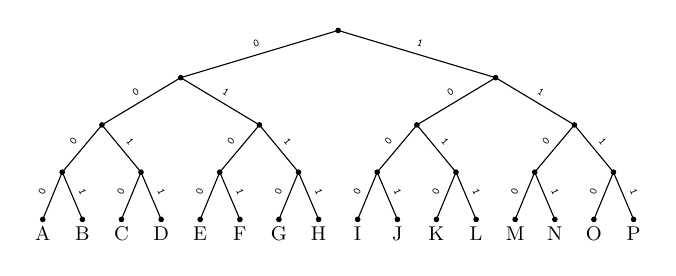
\begin{tikzpicture}[scale=.8,transform shape]
      \draw[fill] (0.0,0.0) circle[radius=1pt] node[below,font=\small] {A};
      \draw[fill] (0.63,0.0) circle[radius=1pt] node[below,font=\small] {B};
      \draw[fill] (1.25,0.0) circle[radius=1pt] node[below,font=\small] {C};
      \draw[fill] (1.88,0.0) circle[radius=1pt] node[below,font=\small] {D};
      \draw[fill] (2.5,0.0) circle[radius=1pt] node[below,font=\small] {E};
      \draw[fill] (3.13,0.0) circle[radius=1pt] node[below,font=\small] {F};
      \draw[fill] (3.75,0.0) circle[radius=1pt] node[below,font=\small] {G};
      \draw[fill] (4.38,0.0) circle[radius=1pt] node[below,font=\small] {H};
      \draw[fill] (5.0,0.0) circle[radius=1pt] node[below,font=\small] {I};
      \draw[fill] (5.63,0.0) circle[radius=1pt] node[below,font=\small] {J};
      \draw[fill] (6.25,0.0) circle[radius=1pt] node[below,font=\small] {K};
      \draw[fill] (6.88,0.0) circle[radius=1pt] node[below,font=\small] {L};
      \draw[fill] (7.5,0.0) circle[radius=1pt] node[below,font=\small] {M};
      \draw[fill] (8.13,0.0) circle[radius=1pt] node[below,font=\small] {N};
      \draw[fill] (8.75,0.0) circle[radius=1pt] node[below,font=\small] {O};
      \draw[fill] (9.38,0.0) circle[radius=1pt] node[below,font=\small] {P};
      \draw (0.0,0.0) -- (0.31,0.75) node[midway,above,sloped,font=\tiny] {\tt 0};
      \draw (0.63,0.0) -- (0.31,0.75) node[midway,above,sloped,font=\tiny] {\tt 1};
      \draw (1.25,0.0) -- (1.56,0.75) node[midway,above,sloped,font=\tiny] {\tt 0};
      \draw (1.88,0.0) -- (1.56,0.75) node[midway,above,sloped,font=\tiny] {\tt 1};
      \draw (2.5,0.0) -- (2.81,0.75) node[midway,above,sloped,font=\tiny] {\tt 0};
      \draw (3.13,0.0) -- (2.81,0.75) node[midway,above,sloped,font=\tiny] {\tt 1};
      \draw (3.75,0.0) -- (4.06,0.75) node[midway,above,sloped,font=\tiny] {\tt 0};
      \draw (4.38,0.0) -- (4.06,0.75) node[midway,above,sloped,font=\tiny] {\tt 1};
      \draw (5.0,0.0) -- (5.31,0.75) node[midway,above,sloped,font=\tiny] {\tt 0};
      \draw (5.63,0.0) -- (5.31,0.75) node[midway,above,sloped,font=\tiny] {\tt 1};
      \draw (6.25,0.0) -- (6.56,0.75) node[midway,above,sloped,font=\tiny] {\tt 0};
      \draw (6.88,0.0) -- (6.56,0.75) node[midway,above,sloped,font=\tiny] {\tt 1};
      \draw (7.5,0.0) -- (7.81,0.75) node[midway,above,sloped,font=\tiny] {\tt 0};
      \draw (8.13,0.0) -- (7.81,0.75) node[midway,above,sloped,font=\tiny] {\tt 1};
      \draw (8.75,0.0) -- (9.06,0.75) node[midway,above,sloped,font=\tiny] {\tt 0};
      \draw (9.38,0.0) -- (9.06,0.75) node[midway,above,sloped,font=\tiny] {\tt 1};
      \draw[fill] (0.31,0.75) circle[radius=1pt];
      \draw[fill] (1.56,0.75) circle[radius=1pt];
      \draw[fill] (2.81,0.75) circle[radius=1pt];
      \draw[fill] (4.06,0.75) circle[radius=1pt];
      \draw[fill] (5.31,0.75) circle[radius=1pt];
      \draw[fill] (6.56,0.75) circle[radius=1pt];
      \draw[fill] (7.81,0.75) circle[radius=1pt];
      \draw[fill] (9.06,0.75) circle[radius=1pt];
      \draw (0.31,0.75) -- (0.94,1.5) node[midway,above,sloped,font=\tiny] {\tt 0};
      \draw (1.56,0.75) -- (0.94,1.5) node[midway,above,sloped,font=\tiny] {\tt 1};
      \draw (2.81,0.75) -- (3.44,1.5) node[midway,above,sloped,font=\tiny] {\tt 0};
      \draw (4.06,0.75) -- (3.44,1.5) node[midway,above,sloped,font=\tiny] {\tt 1};
      \draw (5.31,0.75) -- (5.94,1.5) node[midway,above,sloped,font=\tiny] {\tt 0};
      \draw (6.56,0.75) -- (5.94,1.5) node[midway,above,sloped,font=\tiny] {\tt 1};
      \draw (7.81,0.75) -- (8.44,1.5) node[midway,above,sloped,font=\tiny] {\tt 0};
      \draw (9.06,0.75) -- (8.44,1.5) node[midway,above,sloped,font=\tiny] {\tt 1};
      \draw[fill] (0.94,1.5) circle[radius=1pt];
      \draw[fill] (3.44,1.5) circle[radius=1pt];
      \draw[fill] (5.94,1.5) circle[radius=1pt];
      \draw[fill] (8.44,1.5) circle[radius=1pt];
      \draw (0.94,1.5) -- (2.19,2.25) node[midway,above,sloped,font=\tiny] {\tt 0};
      \draw (3.44,1.5) -- (2.19,2.25) node[midway,above,sloped,font=\tiny] {\tt 1};
      \draw (5.94,1.5) -- (7.19,2.25) node[midway,above,sloped,font=\tiny] {\tt 0};
      \draw (8.44,1.5) -- (7.19,2.25) node[midway,above,sloped,font=\tiny] {\tt 1};
      \draw[fill] (2.19,2.25) circle[radius=1pt];
      \draw[fill] (7.19,2.25) circle[radius=1pt];
      \draw (2.19,2.25) -- (4.69,3.0) node[midway,above,sloped,font=\tiny] {\tt 0};
      \draw (7.19,2.25) -- (4.69,3.0) node[midway,above,sloped,font=\tiny] {\tt 1};
      \draw[fill] (4.69,3.0) circle[radius=1pt];
    \end{tikzpicture}
  \end{center}
  \begin{columns}
    \small
    \column{3cm}
    \begin{center}
      \begin{tabular}{cc}
        \textbf{Letter} & \textbf{Code} \\
        \toprule
        A & \tt 0000 \\
        B & \tt 0001 \\
        C & \tt 0010 \\
        D & \tt 0011 \\
      \end{tabular}
    \end{center}

    \column{3cm}
    \begin{center}
      \begin{tabular}{cc}
        \textbf{Letter} & \textbf{Code} \\
        \toprule
        E & \tt 0100 \\
        F & \tt 0101 \\
        G & \tt 0110 \\
        H & \tt 0111 \\
      \end{tabular}
    \end{center}

    \column{3cm}
    \begin{center}
      \begin{tabular}{cc}
        \textbf{Letter} & \textbf{Code} \\
        \toprule
        I & \tt 1000 \\
        J & \tt 1001 \\
        K & \tt 1010 \\
        L & \tt 1011 \\
      \end{tabular}
    \end{center}

    \column{3cm}
    \begin{center}
      \begin{tabular}{cc}
        \textbf{Letter} & \textbf{Code} \\
        \toprule
        M & \tt 1100 \\
        N & \tt 1101 \\
        O & \tt 1110 \\
        P & \tt 1111 \\
      \end{tabular}
    \end{center}
  \end{columns}
\end{frame}

\begin{frame}
  \frametitle{Modifying the Tree}
  \begin{itemize}
    \item How can we safely modify this tree?
          \vskip4mm
    \item The actual codes do not matter
          \begin{itemize}
            \item Whether A is 0000 or 1111 is not important
          \end{itemize}
          \vskip4mm
    \item What matters to us is
          \begin{itemize}
            \item the \emph{length} of each code
            \item the \emph{unambiguity} of each code
          \end{itemize}
  \end{itemize}
\end{frame}

\begin{frame}
  \frametitle{Swapping Nodes}
  \begin{center}
    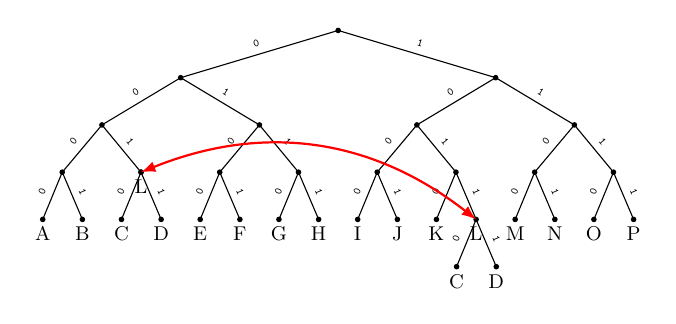
\begin{tikzpicture}[scale=.8,transform shape]
      \draw[fill] (0.0,0.0) circle[radius=1pt] node[below,font=\small] {A};
      \draw[fill] (0.63,0.0) circle[radius=1pt] node[below,font=\small] {B};
      \draw[fill] (2.5,0.0) circle[radius=1pt] node[below,font=\small] {E};
      \draw[fill] (3.13,0.0) circle[radius=1pt] node[below,font=\small] {F};
      \draw[fill] (3.75,0.0) circle[radius=1pt] node[below,font=\small] {G};
      \draw[fill] (4.38,0.0) circle[radius=1pt] node[below,font=\small] {H};
      \draw[fill] (5.0,0.0) circle[radius=1pt] node[below,font=\small] {I};
      \draw[fill] (5.63,0.0) circle[radius=1pt] node[below,font=\small] {J};
      \draw[fill] (6.25,0.0) circle[radius=1pt] node[below,font=\small] {K};
      \draw[fill] (7.5,0.0) circle[radius=1pt] node[below,font=\small] {M};
      \draw[fill] (8.13,0.0) circle[radius=1pt] node[below,font=\small] {N};
      \draw[fill] (8.75,0.0) circle[radius=1pt] node[below,font=\small] {O};
      \draw[fill] (9.38,0.0) circle[radius=1pt] node[below,font=\small] {P};
      \draw (0.0,0.0) -- (0.31,0.75) node[midway,above,sloped,font=\tiny] {\tt 0};
      \draw (0.63,0.0) -- (0.31,0.75) node[midway,above,sloped,font=\tiny] {\tt 1};
      \draw (2.5,0.0) -- (2.81,0.75) node[midway,above,sloped,font=\tiny] {\tt 0};
      \draw (3.13,0.0) -- (2.81,0.75) node[midway,above,sloped,font=\tiny] {\tt 1};
      \draw (3.75,0.0) -- (4.06,0.75) node[midway,above,sloped,font=\tiny] {\tt 0};
      \draw (4.38,0.0) -- (4.06,0.75) node[midway,above,sloped,font=\tiny] {\tt 1};
      \draw (5.0,0.0) -- (5.31,0.75) node[midway,above,sloped,font=\tiny] {\tt 0};
      \draw (5.63,0.0) -- (5.31,0.75) node[midway,above,sloped,font=\tiny] {\tt 1};
      \draw (6.25,0.0) -- (6.56,0.75) node[midway,above,sloped,font=\tiny] {\tt 0};
      \draw (6.88,0.0) -- (6.56,0.75) node[midway,above,sloped,font=\tiny] {\tt 1};
      \draw (7.5,0.0) -- (7.81,0.75) node[midway,above,sloped,font=\tiny] {\tt 0};
      \draw (8.13,0.0) -- (7.81,0.75) node[midway,above,sloped,font=\tiny] {\tt 1};
      \draw (8.75,0.0) -- (9.06,0.75) node[midway,above,sloped,font=\tiny] {\tt 0};
      \draw (9.38,0.0) -- (9.06,0.75) node[midway,above,sloped,font=\tiny] {\tt 1};
      \draw[fill] (0.31,0.75) circle[radius=1pt];
      \draw[fill] (1.56,0.75) circle[radius=1pt];
      \draw[fill] (2.81,0.75) circle[radius=1pt];
      \draw[fill] (4.06,0.75) circle[radius=1pt];
      \draw[fill] (5.31,0.75) circle[radius=1pt];
      \draw[fill] (6.56,0.75) circle[radius=1pt];
      \draw[fill] (7.81,0.75) circle[radius=1pt];
      \draw[fill] (9.06,0.75) circle[radius=1pt];
      \draw (0.31,0.75) -- (0.94,1.5) node[midway,above,sloped,font=\tiny] {\tt 0};
      \draw (1.56,0.75) -- (0.94,1.5) node[midway,above,sloped,font=\tiny] {\tt 1};
      \draw (2.81,0.75) -- (3.44,1.5) node[midway,above,sloped,font=\tiny] {\tt 0};
      \draw (4.06,0.75) -- (3.44,1.5) node[midway,above,sloped,font=\tiny] {\tt 1};
      \draw (5.31,0.75) -- (5.94,1.5) node[midway,above,sloped,font=\tiny] {\tt 0};
      \draw (6.56,0.75) -- (5.94,1.5) node[midway,above,sloped,font=\tiny] {\tt 1};
      \draw (7.81,0.75) -- (8.44,1.5) node[midway,above,sloped,font=\tiny] {\tt 0};
      \draw (9.06,0.75) -- (8.44,1.5) node[midway,above,sloped,font=\tiny] {\tt 1};
      \draw[fill] (0.94,1.5) circle[radius=1pt];
      \draw[fill] (3.44,1.5) circle[radius=1pt];
      \draw[fill] (5.94,1.5) circle[radius=1pt];
      \draw[fill] (8.44,1.5) circle[radius=1pt];
      \draw (0.94,1.5) -- (2.19,2.25) node[midway,above,sloped,font=\tiny] {\tt 0};
      \draw (3.44,1.5) -- (2.19,2.25) node[midway,above,sloped,font=\tiny] {\tt 1};
      \draw (5.94,1.5) -- (7.19,2.25) node[midway,above,sloped,font=\tiny] {\tt 0};
      \draw (8.44,1.5) -- (7.19,2.25) node[midway,above,sloped,font=\tiny] {\tt 1};
      \draw[fill] (2.19,2.25) circle[radius=1pt];
      \draw[fill] (7.19,2.25) circle[radius=1pt];
      \draw (2.19,2.25) -- (4.69,3.0) node[midway,above,sloped,font=\tiny] {\tt 0};
      \draw (7.19,2.25) -- (4.69,3.0) node[midway,above,sloped,font=\tiny] {\tt 1};
      \draw[fill] (4.69,3.0) circle[radius=1pt];

      \visible<handout:1|1-2>{
        \draw[fill] (1.25,0.0) circle[radius=1pt] node[below,font=\small] {C};
        \draw[fill] (1.88,0.0) circle[radius=1pt] node[below,font=\small] {D};
        \draw (1.25,0.0) -- (1.56,0.75) node[midway,above,sloped,font=\tiny] {\tt 0};
        \draw (1.88,0.0) -- (1.56,0.75) node[midway,above,sloped,font=\tiny] {\tt 1};
        \draw[fill] (6.88,0.0) circle[radius=1pt] node[below,font=\small] {L};
      }

      \visible<handout:2|3>{
        \begin{scope}[xshift=-1.56cm,yshift=-0.75cm,xshift=6.88cm]
          \draw[fill] (1.25,0.0) circle[radius=1pt] node[below,font=\small] {C};
          \draw[fill] (1.88,0.0) circle[radius=1pt] node[below,font=\small] {D};
          \draw (1.25,0.0) -- (1.56,0.75) node[midway,above,sloped,font=\tiny] {\tt 0};
          \draw (1.88,0.0) -- (1.56,0.75) node[midway,above,sloped,font=\tiny] {\tt 1};
        \end{scope}

        \draw[fill] (1.56,0.75) circle[radius=1pt] node[below,font=\small] {L};
      }

      \visible<handout:1|2>{
        \draw[latex-latex,red,thick] (1.56,0.75) to [bend left=30] (6.88,0.0);
      }
    \end{tikzpicture}
  \end{center}

  \begin{columns}
    \small
    \column{3cm}
    \begin{center}
      \begin{tabular}{cc}
        \textbf{Letter} & \textbf{Code} \\
        \toprule
        A & \tt 0000 \\
        B & \tt 0001 \\
        C & \tt \alt<1-2>{0010}{\color{red}10110} \\
        D & \tt \alt<1-2>{0011}{\color{red}10111} \\
      \end{tabular}
    \end{center}

    \column{3cm}
    \begin{center}
      \begin{tabular}{cc}
        \textbf{Letter} & \textbf{Code} \\
        \toprule
        E & \tt 0100 \\
        F & \tt 0101 \\
        G & \tt 0110 \\
        H & \tt 0111 \\
      \end{tabular}
    \end{center}

    \column{3cm}
    \begin{center}
      \begin{tabular}{cc}
        \textbf{Letter} & \textbf{Code} \\
        \toprule
        I & \tt 1000 \\
        J & \tt 1001 \\
        K & \tt 1010 \\
        L & \tt \alt<1-2>{1011}{\color{red}001} \\
      \end{tabular}
    \end{center}

    \column{3cm}
    \begin{center}
      \begin{tabular}{cc}
        \textbf{Letter} & \textbf{Code} \\
        \toprule
        M & \tt 1100 \\
        N & \tt 1101 \\
        O & \tt 1110 \\
        P & \tt 1111 \\
      \end{tabular}
    \end{center}
  \end{columns}
\end{frame}

\begin{frame}
  \frametitle{Swapping Nodes}
  \begin{itemize}
    \item We can swap any two nodes in the tree
    \item The resulting code remains unambiguous
    \item The codes have changed
          \begin{itemize}
            \item L's code became 1 bit shorter
            \item C and D's codes became 1 bit longer
            \item Gain 1 bit but lose 2: typical for compression
          \end{itemize}
    \item Goal of swapping:
          \begin{itemize}
            \item Make frequent letters have shorter codes
            \item Sacrifice rarely occurring letters
          \end{itemize}
  \end{itemize}
\end{frame}

\begin{frame}
  \frametitle{Optimal Tree}
  \begin{center} \small
    \begin{tabular}{cc@{\hspace{5mm}}cc@{\hspace{5mm}}cc@{\hspace{5mm}}cc}
      \textbf{Letter} & \textbf{\#} & \textbf{Letter} & \textbf{\#} & \textbf{Letter} & \textbf{\#} & \textbf{Letter} & \textbf{\#} \\
      \toprule
      A & 98 & E & 154 & I & 72 & M & 29 \\
      B & 20 & F & 54 & J & 3 & N & 81 \\
      C & 22 & G & 27 & K & 14 & O & 92 \\
      D & 66 & H & 87 & L & 54 & P & 15 \\
    \end{tabular}
  \end{center}

  \begin{itemize}
    \item E occurs most often
    \item J and P appear least often
    \item We can ``steal'' from J and P and give to E
          \begin{itemize}
            \item E: 3 bits
            \item P, J: 5 bits
          \end{itemize}
  \end{itemize}
\end{frame}

\begin{frame}
  \frametitle{Optimal Tree}
  \begin{overprint}
    \onslide<handout:1|1>
    \begin{center}
      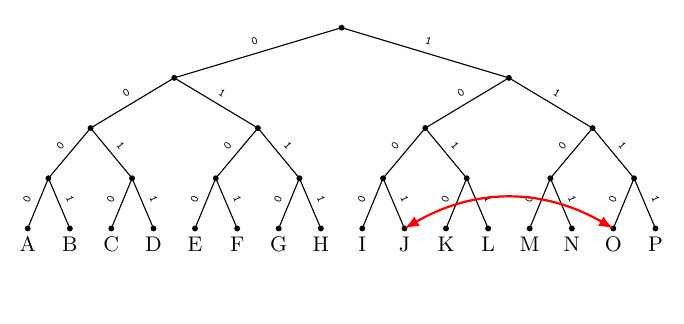
\begin{tikzpicture}[scale=.85,transform shape]
        \path[use as bounding box] (0,-1) rectangle (9.38,3);
        \draw[fill] (0.0,0.0) circle[radius=1pt] node[below,font=\small] {A};
        \draw[fill] (0.63,0.0) circle[radius=1pt] node[below,font=\small] {B};
        \draw[fill] (1.25,0.0) circle[radius=1pt] node[below,font=\small] {C};
        \draw[fill] (1.88,0.0) circle[radius=1pt] node[below,font=\small] {D};
        \draw[fill] (2.5,0.0) circle[radius=1pt] node[below,font=\small] {E};
        \draw[fill] (3.13,0.0) circle[radius=1pt] node[below,font=\small] {F};
        \draw[fill] (3.75,0.0) circle[radius=1pt] node[below,font=\small] {G};
        \draw[fill] (4.38,0.0) circle[radius=1pt] node[below,font=\small] {H};
        \draw[fill] (5.0,0.0) circle[radius=1pt] node[below,font=\small] {I};
        \draw[fill] (5.63,0.0) circle[radius=1pt] node[below,font=\small] {J};
        \draw[fill] (6.25,0.0) circle[radius=1pt] node[below,font=\small] {K};
        \draw[fill] (6.88,0.0) circle[radius=1pt] node[below,font=\small] {L};
        \draw[fill] (7.5,0.0) circle[radius=1pt] node[below,font=\small] {M};
        \draw[fill] (8.13,0.0) circle[radius=1pt] node[below,font=\small] {N};
        \draw[fill] (8.75,0.0) circle[radius=1pt] node[below,font=\small] {O};
        \draw[fill] (9.38,0.0) circle[radius=1pt] node[below,font=\small] {P};
        \draw (0.0,0.0) -- (0.31,0.75) node[midway,above,sloped,font=\tiny] {\tt 0};
        \draw (0.63,0.0) -- (0.31,0.75) node[midway,above,sloped,font=\tiny] {\tt 1};
        \draw (1.25,0.0) -- (1.56,0.75) node[midway,above,sloped,font=\tiny] {\tt 0};
        \draw (1.88,0.0) -- (1.56,0.75) node[midway,above,sloped,font=\tiny] {\tt 1};
        \draw (2.5,0.0) -- (2.81,0.75) node[midway,above,sloped,font=\tiny] {\tt 0};
        \draw (3.13,0.0) -- (2.81,0.75) node[midway,above,sloped,font=\tiny] {\tt 1};
        \draw (3.75,0.0) -- (4.06,0.75) node[midway,above,sloped,font=\tiny] {\tt 0};
        \draw (4.38,0.0) -- (4.06,0.75) node[midway,above,sloped,font=\tiny] {\tt 1};
        \draw (5.0,0.0) -- (5.31,0.75) node[midway,above,sloped,font=\tiny] {\tt 0};
        \draw (5.63,0.0) -- (5.31,0.75) node[midway,above,sloped,font=\tiny] {\tt 1};
        \draw (6.25,0.0) -- (6.56,0.75) node[midway,above,sloped,font=\tiny] {\tt 0};
        \draw (6.88,0.0) -- (6.56,0.75) node[midway,above,sloped,font=\tiny] {\tt 1};
        \draw (7.5,0.0) -- (7.81,0.75) node[midway,above,sloped,font=\tiny] {\tt 0};
        \draw (8.13,0.0) -- (7.81,0.75) node[midway,above,sloped,font=\tiny] {\tt 1};
        \draw (8.75,0.0) -- (9.06,0.75) node[midway,above,sloped,font=\tiny] {\tt 0};
        \draw (9.38,0.0) -- (9.06,0.75) node[midway,above,sloped,font=\tiny] {\tt 1};
        \draw[fill] (0.31,0.75) circle[radius=1pt];
        \draw[fill] (1.56,0.75) circle[radius=1pt];
        \draw[fill] (2.81,0.75) circle[radius=1pt];
        \draw[fill] (4.06,0.75) circle[radius=1pt];
        \draw[fill] (5.31,0.75) circle[radius=1pt];
        \draw[fill] (6.56,0.75) circle[radius=1pt];
        \draw[fill] (7.81,0.75) circle[radius=1pt];
        \draw[fill] (9.06,0.75) circle[radius=1pt];
        \draw (0.31,0.75) -- (0.94,1.5) node[midway,above,sloped,font=\tiny] {\tt 0};
        \draw (1.56,0.75) -- (0.94,1.5) node[midway,above,sloped,font=\tiny] {\tt 1};
        \draw (2.81,0.75) -- (3.44,1.5) node[midway,above,sloped,font=\tiny] {\tt 0};
        \draw (4.06,0.75) -- (3.44,1.5) node[midway,above,sloped,font=\tiny] {\tt 1};
        \draw (5.31,0.75) -- (5.94,1.5) node[midway,above,sloped,font=\tiny] {\tt 0};
        \draw (6.56,0.75) -- (5.94,1.5) node[midway,above,sloped,font=\tiny] {\tt 1};
        \draw (7.81,0.75) -- (8.44,1.5) node[midway,above,sloped,font=\tiny] {\tt 0};
        \draw (9.06,0.75) -- (8.44,1.5) node[midway,above,sloped,font=\tiny] {\tt 1};
        \draw[fill] (0.94,1.5) circle[radius=1pt];
        \draw[fill] (3.44,1.5) circle[radius=1pt];
        \draw[fill] (5.94,1.5) circle[radius=1pt];
        \draw[fill] (8.44,1.5) circle[radius=1pt];
        \draw (0.94,1.5) -- (2.19,2.25) node[midway,above,sloped,font=\tiny] {\tt 0};
        \draw (3.44,1.5) -- (2.19,2.25) node[midway,above,sloped,font=\tiny] {\tt 1};
        \draw (5.94,1.5) -- (7.19,2.25) node[midway,above,sloped,font=\tiny] {\tt 0};
        \draw (8.44,1.5) -- (7.19,2.25) node[midway,above,sloped,font=\tiny] {\tt 1};
        \draw[fill] (2.19,2.25) circle[radius=1pt];
        \draw[fill] (7.19,2.25) circle[radius=1pt];
        \draw (2.19,2.25) -- (4.69,3.0) node[midway,above,sloped,font=\tiny] {\tt 0};
        \draw (7.19,2.25) -- (4.69,3.0) node[midway,above,sloped,font=\tiny] {\tt 1};
        \draw[fill] (4.69,3.0) circle[radius=1pt];

        \draw[thick,red,latex-latex] (5.63,0.0) to[bend left=30] (8.75,0.0);
      \end{tikzpicture}
    \end{center}

    \onslide<handout:2-3|2-3>
    \begin{center}
      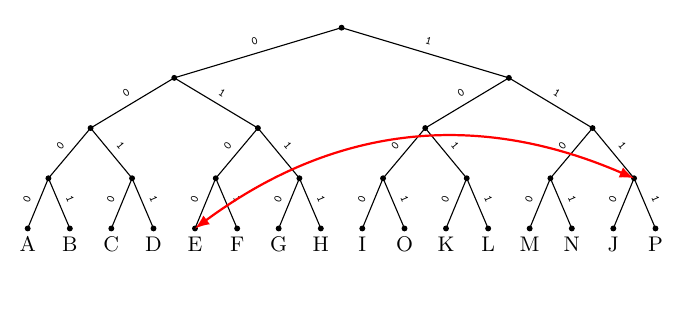
\begin{tikzpicture}[scale=.85,transform shape]
        \path[use as bounding box] (0,-1) rectangle (9.38,3);
        \draw[fill] (0.0,0.0) circle[radius=1pt] node[below,font=\small] {A};
        \draw[fill] (0.63,0.0) circle[radius=1pt] node[below,font=\small] {B};
        \draw[fill] (1.25,0.0) circle[radius=1pt] node[below,font=\small] {C};
        \draw[fill] (1.88,0.0) circle[radius=1pt] node[below,font=\small] {D};
        \draw[fill] (2.5,0.0) circle[radius=1pt] node[below,font=\small] {E};
        \draw[fill] (3.13,0.0) circle[radius=1pt] node[below,font=\small] {F};
        \draw[fill] (3.75,0.0) circle[radius=1pt] node[below,font=\small] {G};
        \draw[fill] (4.38,0.0) circle[radius=1pt] node[below,font=\small] {H};
        \draw[fill] (5.0,0.0) circle[radius=1pt] node[below,font=\small] {I};
        \draw[fill] (5.63,0.0) circle[radius=1pt] node[below,font=\small] {O};
        \draw[fill] (6.25,0.0) circle[radius=1pt] node[below,font=\small] {K};
        \draw[fill] (6.88,0.0) circle[radius=1pt] node[below,font=\small] {L};
        \draw[fill] (7.5,0.0) circle[radius=1pt] node[below,font=\small] {M};
        \draw[fill] (8.13,0.0) circle[radius=1pt] node[below,font=\small] {N};
        \draw[fill] (8.75,0.0) circle[radius=1pt] node[below,font=\small] {J};
        \draw[fill] (9.38,0.0) circle[radius=1pt] node[below,font=\small] {P};
        \draw (0.0,0.0) -- (0.31,0.75) node[midway,above,sloped,font=\tiny] {\tt 0};
        \draw (0.63,0.0) -- (0.31,0.75) node[midway,above,sloped,font=\tiny] {\tt 1};
        \draw (1.25,0.0) -- (1.56,0.75) node[midway,above,sloped,font=\tiny] {\tt 0};
        \draw (1.88,0.0) -- (1.56,0.75) node[midway,above,sloped,font=\tiny] {\tt 1};
        \draw (2.5,0.0) -- (2.81,0.75) node[midway,above,sloped,font=\tiny] {\tt 0};
        \draw (3.13,0.0) -- (2.81,0.75) node[midway,above,sloped,font=\tiny] {\tt 1};
        \draw (3.75,0.0) -- (4.06,0.75) node[midway,above,sloped,font=\tiny] {\tt 0};
        \draw (4.38,0.0) -- (4.06,0.75) node[midway,above,sloped,font=\tiny] {\tt 1};
        \draw (5.0,0.0) -- (5.31,0.75) node[midway,above,sloped,font=\tiny] {\tt 0};
        \draw (5.63,0.0) -- (5.31,0.75) node[midway,above,sloped,font=\tiny] {\tt 1};
        \draw (6.25,0.0) -- (6.56,0.75) node[midway,above,sloped,font=\tiny] {\tt 0};
        \draw (6.88,0.0) -- (6.56,0.75) node[midway,above,sloped,font=\tiny] {\tt 1};
        \draw (7.5,0.0) -- (7.81,0.75) node[midway,above,sloped,font=\tiny] {\tt 0};
        \draw (8.13,0.0) -- (7.81,0.75) node[midway,above,sloped,font=\tiny] {\tt 1};
        \draw (8.75,0.0) -- (9.06,0.75) node[midway,above,sloped,font=\tiny] {\tt 0};
        \draw (9.38,0.0) -- (9.06,0.75) node[midway,above,sloped,font=\tiny] {\tt 1};
        \draw[fill] (0.31,0.75) circle[radius=1pt];
        \draw[fill] (1.56,0.75) circle[radius=1pt];
        \draw[fill] (2.81,0.75) circle[radius=1pt];
        \draw[fill] (4.06,0.75) circle[radius=1pt];
        \draw[fill] (5.31,0.75) circle[radius=1pt];
        \draw[fill] (6.56,0.75) circle[radius=1pt];
        \draw[fill] (7.81,0.75) circle[radius=1pt];
        \draw[fill] (9.06,0.75) circle[radius=1pt];
        \draw (0.31,0.75) -- (0.94,1.5) node[midway,above,sloped,font=\tiny] {\tt 0};
        \draw (1.56,0.75) -- (0.94,1.5) node[midway,above,sloped,font=\tiny] {\tt 1};
        \draw (2.81,0.75) -- (3.44,1.5) node[midway,above,sloped,font=\tiny] {\tt 0};
        \draw (4.06,0.75) -- (3.44,1.5) node[midway,above,sloped,font=\tiny] {\tt 1};
        \draw (5.31,0.75) -- (5.94,1.5) node[midway,above,sloped,font=\tiny] {\tt 0};
        \draw (6.56,0.75) -- (5.94,1.5) node[midway,above,sloped,font=\tiny] {\tt 1};
        \draw (7.81,0.75) -- (8.44,1.5) node[midway,above,sloped,font=\tiny] {\tt 0};
        \draw (9.06,0.75) -- (8.44,1.5) node[midway,above,sloped,font=\tiny] {\tt 1};
        \draw[fill] (0.94,1.5) circle[radius=1pt];
        \draw[fill] (3.44,1.5) circle[radius=1pt];
        \draw[fill] (5.94,1.5) circle[radius=1pt];
        \draw[fill] (8.44,1.5) circle[radius=1pt];
        \draw (0.94,1.5) -- (2.19,2.25) node[midway,above,sloped,font=\tiny] {\tt 0};
        \draw (3.44,1.5) -- (2.19,2.25) node[midway,above,sloped,font=\tiny] {\tt 1};
        \draw (5.94,1.5) -- (7.19,2.25) node[midway,above,sloped,font=\tiny] {\tt 0};
        \draw (8.44,1.5) -- (7.19,2.25) node[midway,above,sloped,font=\tiny] {\tt 1};
        \draw[fill] (2.19,2.25) circle[radius=1pt];
        \draw[fill] (7.19,2.25) circle[radius=1pt];
        \draw (2.19,2.25) -- (4.69,3.0) node[midway,above,sloped,font=\tiny] {\tt 0};
        \draw (7.19,2.25) -- (4.69,3.0) node[midway,above,sloped,font=\tiny] {\tt 1};
        \draw[fill] (4.69,3.0) circle[radius=1pt];

        \only<handout:3|3>{
          \draw[thick,red,latex-latex] (2.5,0.0) to[bend left=30] (9.06,0.75);
        }
      \end{tikzpicture}
    \end{center}

    \onslide<handout:4|4->
    \begin{center}
      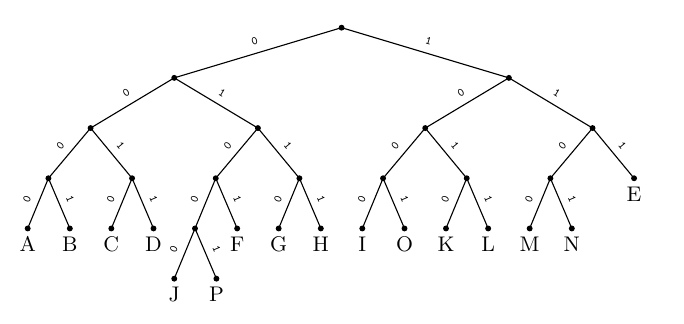
\begin{tikzpicture}[scale=.85,transform shape]
        \path[use as bounding box] (0,-1) rectangle (9.38,3);
        \draw[fill] (0.0,0.0) circle[radius=1pt] node[below,font=\small] {A};
        \draw[fill] (0.63,0.0) circle[radius=1pt] node[below,font=\small] {B};
        \draw[fill] (1.25,0.0) circle[radius=1pt] node[below,font=\small] {C};
        \draw[fill] (1.88,0.0) circle[radius=1pt] node[below,font=\small] {D};
        \draw[fill] (3.13,0.0) circle[radius=1pt] node[below,font=\small] {F};
        \draw[fill] (3.75,0.0) circle[radius=1pt] node[below,font=\small] {G};
        \draw[fill] (4.38,0.0) circle[radius=1pt] node[below,font=\small] {H};
        \draw[fill] (5.0,0.0) circle[radius=1pt] node[below,font=\small] {I};
        \draw[fill] (5.63,0.0) circle[radius=1pt] node[below,font=\small] {O};
        \draw[fill] (6.25,0.0) circle[radius=1pt] node[below,font=\small] {K};
        \draw[fill] (6.88,0.0) circle[radius=1pt] node[below,font=\small] {L};
        \draw[fill] (7.5,0.0) circle[radius=1pt] node[below,font=\small] {M};
        \draw[fill] (8.13,0.0) circle[radius=1pt] node[below,font=\small] {N};
        \draw (0.0,0.0) -- (0.31,0.75) node[midway,above,sloped,font=\tiny] {\tt 0};
        \draw (0.63,0.0) -- (0.31,0.75) node[midway,above,sloped,font=\tiny] {\tt 1};
        \draw (1.25,0.0) -- (1.56,0.75) node[midway,above,sloped,font=\tiny] {\tt 0};
        \draw (1.88,0.0) -- (1.56,0.75) node[midway,above,sloped,font=\tiny] {\tt 1};
        \draw (3.13,0.0) -- (2.81,0.75) node[midway,above,sloped,font=\tiny] {\tt 1};
        \draw (3.75,0.0) -- (4.06,0.75) node[midway,above,sloped,font=\tiny] {\tt 0};
        \draw (4.38,0.0) -- (4.06,0.75) node[midway,above,sloped,font=\tiny] {\tt 1};
        \draw (5.0,0.0) -- (5.31,0.75) node[midway,above,sloped,font=\tiny] {\tt 0};
        \draw (5.63,0.0) -- (5.31,0.75) node[midway,above,sloped,font=\tiny] {\tt 1};
        \draw (6.25,0.0) -- (6.56,0.75) node[midway,above,sloped,font=\tiny] {\tt 0};
        \draw (6.88,0.0) -- (6.56,0.75) node[midway,above,sloped,font=\tiny] {\tt 1};
        \draw (7.5,0.0) -- (7.81,0.75) node[midway,above,sloped,font=\tiny] {\tt 0};
        \draw (8.13,0.0) -- (7.81,0.75) node[midway,above,sloped,font=\tiny] {\tt 1};
        \draw[fill] (0.31,0.75) circle[radius=1pt];
        \draw[fill] (1.56,0.75) circle[radius=1pt];
        \draw[fill] (2.81,0.75) circle[radius=1pt];
        \draw[fill] (4.06,0.75) circle[radius=1pt];
        \draw[fill] (5.31,0.75) circle[radius=1pt];
        \draw[fill] (6.56,0.75) circle[radius=1pt];
        \draw[fill] (7.81,0.75) circle[radius=1pt];
        \draw (0.31,0.75) -- (0.94,1.5) node[midway,above,sloped,font=\tiny] {\tt 0};
        \draw (1.56,0.75) -- (0.94,1.5) node[midway,above,sloped,font=\tiny] {\tt 1};
        \draw (2.81,0.75) -- (3.44,1.5) node[midway,above,sloped,font=\tiny] {\tt 0};
        \draw (4.06,0.75) -- (3.44,1.5) node[midway,above,sloped,font=\tiny] {\tt 1};
        \draw (5.31,0.75) -- (5.94,1.5) node[midway,above,sloped,font=\tiny] {\tt 0};
        \draw (6.56,0.75) -- (5.94,1.5) node[midway,above,sloped,font=\tiny] {\tt 1};
        \draw (7.81,0.75) -- (8.44,1.5) node[midway,above,sloped,font=\tiny] {\tt 0};
        \draw (9.06,0.75) -- (8.44,1.5) node[midway,above,sloped,font=\tiny] {\tt 1};
        \draw[fill] (0.94,1.5) circle[radius=1pt];
        \draw[fill] (3.44,1.5) circle[radius=1pt];
        \draw[fill] (5.94,1.5) circle[radius=1pt];
        \draw[fill] (8.44,1.5) circle[radius=1pt];
        \draw (0.94,1.5) -- (2.19,2.25) node[midway,above,sloped,font=\tiny] {\tt 0};
        \draw (3.44,1.5) -- (2.19,2.25) node[midway,above,sloped,font=\tiny] {\tt 1};
        \draw (5.94,1.5) -- (7.19,2.25) node[midway,above,sloped,font=\tiny] {\tt 0};
        \draw (8.44,1.5) -- (7.19,2.25) node[midway,above,sloped,font=\tiny] {\tt 1};
        \draw[fill] (2.19,2.25) circle[radius=1pt];
        \draw[fill] (7.19,2.25) circle[radius=1pt];
        \draw (2.19,2.25) -- (4.69,3.0) node[midway,above,sloped,font=\tiny] {\tt 0};
        \draw (7.19,2.25) -- (4.69,3.0) node[midway,above,sloped,font=\tiny] {\tt 1};
        \draw[fill] (4.69,3.0) circle[radius=1pt];
        \draw (2.5,0.0) -- (2.81,0.75) node[midway,above,sloped,font=\tiny] {\tt 0};

        \begin{scope}[xshift=-9.06cm,xshift=2.5cm,yshift=-0.75cm]
          \draw[fill] (8.75,0.0) circle[radius=1pt] node[below,font=\small] {J};
          \draw[fill] (9.38,0.0) circle[radius=1pt] node[below,font=\small] {P};
          \draw (8.75,0.0) -- (9.06,0.75) node[midway,above,sloped,font=\tiny] {\tt 0};
          \draw (9.38,0.0) -- (9.06,0.75) node[midway,above,sloped,font=\tiny] {\tt 1};
        \draw[fill] (9.06,0.75) circle[radius=1pt];
        \end{scope}
        \draw[fill] (9.06,0.75) circle[radius=1pt] node[below,font=\small] {E};
      \end{tikzpicture}
    \end{center}
  \end{overprint}
  \begin{itemize}
    \item<handout:1-|1-> We want to make E shorter and P, J longer
    \item<handout:1-|1-> We need to put P and J together somehow
    \item<handout:3-|3-> We can now swap E with P,J
    \item<handout:4|5> New codes: E=111, J=01000, P=01001
  \end{itemize}
\end{frame}

\begin{frame}
  \frametitle{Optimal Tree}
  \begin{itemize}
    \item Is this new tree optimal?
    \item We could make E two bits long by sacrificing other letters
    \item We should perhaps also consider making T and A shorter
    \item In order to find the best, we need a way to compare trees
    \item Can we associate a metric with each tree?
  \end{itemize}
\end{frame}

\begin{frame}
  \frametitle{``Measuring'' Tree}
  \begin{itemize}
    \item Given a tree, we know how many bits each letter requires
    \item We can compute how long the compressed file would be
    \item This is exactly what we want to minimise
    \item Approach to finding optimal tree:
          \begin{itemize}
            \item Consider all trees
            \item Picking the one with the smallest file size
          \end{itemize}
    \item Hardly efficient
    \item Luckily, Huffman developed algorithm to find optimal tree
  \end{itemize}
\end{frame}

\begin{frame}
  \frametitle{Building Huffman Tree}
  \begin{itemize}
    \item Create a leaf node for each byte
    \item Each node has a weight equal to the frequency of this byte
    \item Repeat until there is one node left:
          \begin{itemize}
            \item Take the two nodes with the least weight
            \item Join them in a new node
            \item This node's weight equals the sum of its children
          \end{itemize}
  \end{itemize}
\end{frame}

\begin{frame}
  \frametitle{Building Huffman Tree: Example}
  \begin{center} \small
    \begin{tabular}{cc@{\hspace{5mm}}cc}
      \textbf{Letter} & \textbf{\#} & \textbf{Letter} & \textbf{\#} \\
      \toprule
      A & 98 & E & 154 \\
      B & 20 & F & 54 \\
      C & 22 & G & 27 \\
      D & 66 & H & 87 \\
    \end{tabular}
  \end{center}
  \vskip5mm
  \begin{center}
    \begin{tikzpicture}[node/.style={draw,circle,minimum size=0.75cm,font=\tiny}]
      \only<handout:1|1>{
        \foreach[count=\i] \letter/\frequency in {A/98,B/20,C/22,D/66,E/154,F/54,G/27,H/87} {
          \node[node] (node) at (\i,0) {\frequency};
          \node[anchor=north,font=\tiny] at (node.south) {\letter};
        }
      }
      \only<handout:2|2>{
        \foreach[count=\i] \letter/\frequency in {B/20,C/22,G/27,F/54,D/66,H/87,A/98,E/154} {
          \node[node] (node) at (\i,0) {\frequency};
          \node[anchor=north,font=\tiny] at (node.south) {\letter};
        }
      }
    \end{tikzpicture}
  \end{center}
  \visible<2>{
    \begin{center}
      Ordered by weight
    \end{center}
  }
\end{frame}

\begin{frame}
  \frametitle{Building Huffman Tree: Example}
  \begin{center}
    \begin{tikzpicture}[node/.style={draw,circle,minimum size=0.75cm,font=\tiny}]
      \path[use as bounding box] (-1,-1) rectangle (8,1);

      \node[node] (B) at (0,0) {20};
      \node[anchor=north,font=\tiny] at (B.south) {B};

      \node[node] (C) at (1,0) {22};
      \node[anchor=north,font=\tiny] at (C.south) {C};

      \node[node] (G) at (2,0) {27};
      \node[anchor=north,font=\tiny] at (G.south) {G};

      \node[node] (F) at (3,0) {54};
      \node[anchor=north,font=\tiny] at (F.south) {F};

      \node[node] (D) at (4,0) {66};
      \node[anchor=north,font=\tiny] at (D.south) {D};

      \node[node] (H) at (5,0) {87};
      \node[anchor=north,font=\tiny] at (H.south) {H};

      \node[node] (A) at (6,0) {98};
      \node[anchor=north,font=\tiny] at (A.south) {A};

      \node[node] (E) at (7,0) {154};
      \node[anchor=north,font=\tiny] at (E.south) {E};

      \visible<2->{
        \node[node] (BC) at ($ (B) ! 0.5 ! (C) + (0,1) $) {42};
        \draw (BC) -- (B);
        \draw (BC) -- (C);
      }
    \end{tikzpicture}
  \end{center}
\end{frame}

\begin{frame}
  \frametitle{Building Huffman Tree: Example}
  \begin{center}
    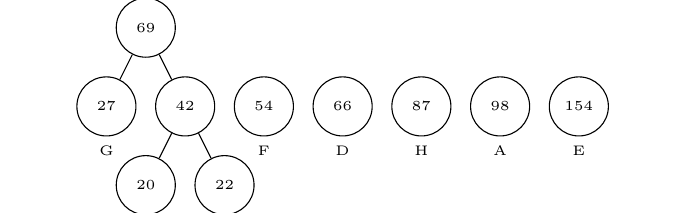
\begin{tikzpicture}[node/.style={draw,circle,minimum size=0.75cm,font=\tiny}]
      \path[use as bounding box] (-1,-1) rectangle (7,1);

      \node[node] (G) at (0,0) {27};
      \node[anchor=north,font=\tiny] at (G.south) {G};

      \node[node] (BC) at (1,0) {42};

      \node[node] (F) at (2,0) {54};
      \node[anchor=north,font=\tiny] at (F.south) {F};

      \node[node] (D) at (3,0) {66};
      \node[anchor=north,font=\tiny] at (D.south) {D};

      \node[node] (H) at (4,0) {87};
      \node[anchor=north,font=\tiny] at (H.south) {H};

      \node[node] (A) at (5,0) {98};
      \node[anchor=north,font=\tiny] at (A.south) {A};

      \node[node] (E) at (6,0) {154};
      \node[anchor=north,font=\tiny] at (E.south) {E};

      \node[node] (B) at (0.5,-1) {20};
      \node[anchor=north,font=\tiny] at (B.south) {B};

      \node[node] (C) at (1.5,-1) {22};
      \node[anchor=north,font=\tiny] at (C.south) {C};

      \draw (BC) -- (B);
      \draw (BC) -- (C);

      \visible<2->{
        \node[node] (GBC) at (0.5,1) {69};
        \draw (GBC) -- (G);
        \draw (GBC) -- (BC);
      }
    \end{tikzpicture}
  \end{center}
\end{frame}

\begin{frame}
  \frametitle{Building Huffman Tree: Example}
  \begin{center}
    \begin{tikzpicture}[node/.style={draw,circle,minimum size=0.75cm,font=\tiny}]
      \path[use as bounding box] (-1,-1) rectangle (6,1);

      \node[node] (F) at (0,0) {54};
      \node[anchor=north,font=\tiny] at (F.south) {F};

      \node[node] (D) at (1,0) {66};
      \node[anchor=north,font=\tiny] at (D.south) {D};

      \node[node] (GBC) at (2,0) {69};

      \node[node] (G) at ($ (GBC) + (-0.5,-1) $) {27};
      \node[anchor=north,font=\tiny] at (G.south) {G};

      \node[node] (BC) at ($ (GBC) + (0.5,-1) $) {42};

      \node[node] (B) at ($ (BC) + (-0.5,-1) $) {20};
      \node[anchor=north,font=\tiny] at (B.south) {B};

      \node[node] (C) at ($ (BC) + (0.5,-1) $) {22};
      \node[anchor=north,font=\tiny] at (C.south) {C};

      \draw (BC) -- (B);
      \draw (BC) -- (C);

      \draw (GBC) -- (G);
      \draw (GBC) -- (BC);

      \node[node] (H) at (3,0) {87};
      \node[anchor=north,font=\tiny] at (H.south) {H};

      \node[node] (A) at (4,0) {98};
      \node[anchor=north,font=\tiny] at (A.south) {A};

      \node[node] (E) at (5,0) {154};
      \node[anchor=north,font=\tiny] at (E.south) {E};

      \visible<2->{
        \node[node] (FD) at (0.5,1) {120};
        \draw (FD) -- (F);
        \draw (FD) -- (D);
      }
    \end{tikzpicture}
  \end{center}
\end{frame}

\begin{frame}
  \frametitle{Building Huffman Tree: Example}
  \begin{center}
    \begin{tikzpicture}[node/.style={draw,circle,minimum size=0.75cm,font=\tiny}]
      \path[use as bounding box] (-1,-1) rectangle (5,1);

      \node[node] (GBC) at (0,0) {69};

      \node[node] (G) at ($ (GBC) + (-0.5,-1) $) {27};
      \node[anchor=north,font=\tiny] at (G.south) {G};

      \node[node] (BC) at ($ (GBC) + (0.5,-1) $) {42};

      \node[node] (B) at ($ (BC) + (-0.5,-1) $) {20};
      \node[anchor=north,font=\tiny] at (B.south) {B};

      \node[node] (C) at ($ (BC) + (0.5,-1) $) {22};
      \node[anchor=north,font=\tiny] at (C.south) {C};

      \node[node] (H) at (1,0) {87};
      \node[anchor=north,font=\tiny] at (H.south) {H};

      \draw (BC) -- (B);
      \draw (BC) -- (C);

      \draw (GBC) -- (G);
      \draw (GBC) -- (BC);

      \node[node] (A) at (2,0) {98};
      \node[anchor=north,font=\tiny] at (A.south) {A};

      \node[node] (FD) at (3,0) {120};

      \node[node] (F) at ($ (FD) + (-0.5,-1) $) {54};
      \node[anchor=north,font=\tiny] at (F.south) {F};

      \node[node] (D) at ($ (FD) + (0.5,-1) $) {66};
      \node[anchor=north,font=\tiny] at (D.south) {D};

      \draw (FD) -- (F);
      \draw (FD) -- (D);

      \node[node] (E) at (4,0) {154};
      \node[anchor=north,font=\tiny] at (E.south) {E};

      \visible<2->{
        \node[node] (GBCH) at (0.5,1) {156};
        \draw (GBCH) -- (GBC);
        \draw (GBCH) -- (H);
      }
    \end{tikzpicture}
  \end{center}
\end{frame}

\begin{frame}
  \frametitle{Building Huffman Tree: Example}
  \begin{center}
    \begin{tikzpicture}[node/.style={draw,circle,minimum size=0.75cm,font=\tiny}]
      \path[use as bounding box] (-1,-1) rectangle (4,1);

      \node[node] (A) at (0,0) {98};
      \node[anchor=north,font=\tiny] at (A.south) {A};

      \node[node] (FD) at (1,0) {120};

      \node[node] (F) at ($ (FD) + (-0.5,-1) $) {54};
      \node[anchor=north,font=\tiny] at (F.south) {F};

      \node[node] (D) at ($ (FD) + (0.5,-1) $) {66};
      \node[anchor=north,font=\tiny] at (D.south) {D};

      \draw (FD) -- (F);
      \draw (FD) -- (D);

      \node[node] (E) at (2,0) {154};
      \node[anchor=north,font=\tiny] at (E.south) {E};

      \node[node] (GBCH) at (3,0) {156};

      \node[node] (GBC) at ($ (GBCH) + (-0.5,-1) $) {69};

      \node[node] (G) at ($ (GBC) + (-0.5,-1) $) {27};
      \node[anchor=north,font=\tiny] at (G.south) {G};

      \node[node] (BC) at ($ (GBC) + (0.5,-1) $) {42};

      \node[node] (B) at ($ (BC) + (-0.5,-1) $) {20};
      \node[anchor=north,font=\tiny] at (B.south) {B};

      \node[node] (C) at ($ (BC) + (0.5,-1) $) {22};
      \node[anchor=north,font=\tiny] at (C.south) {C};

      \node[node] (H) at ($ (GBCH) + (0.5,-1) $) {87};
      \node[anchor=north,font=\tiny] at (H.south) {H};

      \draw (BC) -- (B);
      \draw (BC) -- (C);

      \draw (GBC) -- (G);
      \draw (GBC) -- (BC);

      \draw (GBCH) -- (GBC);
      \draw (GBCH) -- (H);

      \visible<2->{
        \node[node] (AFD) at (0.5,1) {218};
        \draw (AFD) -- (A);
        \draw (AFD) -- (FD);
      }

      \visible<3->{
        \node[node] (EGBCH) at (2.5,1) {310};
        \draw (EGBCH) -- (E);
        \draw (EGBCH) -- (GBCH);
      }

      \visible<4->{
        \node[node] (root) at (1.5,2) {528};
        \draw (root) -- (AFD);
        \draw (root) -- (EGBCH);
      }
    \end{tikzpicture}
  \end{center}
\end{frame}

\begin{frame}
  \frametitle{Building Huffman Tree: Example}
  \begin{columns}
    \column{5cm}
    \begin{center}
      \begin{tikzpicture}[node/.style={draw,circle,minimum size=0.75cm,font=\tiny},
                          label/.style={font=\tiny,midway,above,sloped}]
        \node[node] (A) at (0,0) {98};
        \node[anchor=north,font=\tiny] at (A.south) {A};

        \node[node] (FD) at (1,0) {120};

        \node[node] (F) at ($ (FD) + (-0.5,-1) $) {54};
        \node[anchor=north,font=\tiny] at (F.south) {F};

        \node[node] (D) at ($ (FD) + (0.5,-1) $) {66};
        \node[anchor=north,font=\tiny] at (D.south) {D};

        \draw (FD) -- (F) node[label] {0};
        \draw (FD) -- (D) node[label] {1};

        \node[node] (E) at (2,0) {154};
        \node[anchor=north,font=\tiny] at (E.south) {E};

        \node[node] (GBCH) at (3,0) {156};

        \node[node] (GBC) at ($ (GBCH) + (-0.5,-1) $) {69};

        \node[node] (G) at ($ (GBC) + (-0.5,-1) $) {27};
        \node[anchor=north,font=\tiny] at (G.south) {G};

        \node[node] (BC) at ($ (GBC) + (0.5,-1) $) {42};

        \node[node] (B) at ($ (BC) + (-0.5,-1) $) {20};
        \node[anchor=north,font=\tiny] at (B.south) {B};

        \node[node] (C) at ($ (BC) + (0.5,-1) $) {22};
        \node[anchor=north,font=\tiny] at (C.south) {C};

        \node[node] (H) at ($ (GBCH) + (0.5,-1) $) {87};
        \node[anchor=north,font=\tiny] at (H.south) {H};

        \draw (BC) -- (B) node[label] {0};
        \draw (BC) -- (C) node[label] {1};

        \draw (GBC) -- (G) node[label] {0};
        \draw (GBC) -- (BC) node[label] {1};

        \draw (GBCH) -- (GBC) node[label] {0};
        \draw (GBCH) -- (H) node[label] {1};

        \node[node] (AFD) at (0.5,1) {218};
        \draw (AFD) -- (A) node[label] {0};
        \draw (AFD) -- (FD) node[label] {1};

        \node[node] (EGBCH) at (2.5,1) {310};
        \draw (EGBCH) -- (E) node[label] {0};
        \draw (EGBCH) -- (GBCH) node[label] {1};

        \node[node] (root) at (1.5,2) {528};
        \draw (root) -- (AFD) node[label] {0};
        \draw (root) -- (EGBCH) node[label] {1};
      \end{tikzpicture}
    \end{center}
      
    \column{5cm}
    \begin{center}
      \begin{tabular}{cc}
        \textbf{Letter} & \textbf{Code} \\
        \toprule
        A & 00 \\
        B & 11010 \\
        C & 11011 \\
        D & 011 \\
        E & 10 \\
        F & 010 \\
        G & 1100 \\
        H & 111 \\
      \end{tabular}
    \end{center}
  \end{columns}
\end{frame}

\begin{frame}
  \frametitle{Huffman Compression}
  \begin{enumerate}
    \item Count the frequency of all bytes
    \item Build Huffman tree
    \item Derive code table (byte to code)
    \item Write Huffman tree to file (decompressor needs this information)
    \item Write encoded bytes to file
    \item Is it possible to omit Huffman tree in compressed file? \cake
  \end{enumerate}
\end{frame}


\end{document}


%%% Local Variables:
%%% mode: latex
%%% TeX-master: "compression-huffman"
%%% End:
